\documentclass[a4paper]{article}
\usepackage{amssymb}
\usepackage{graphicx}
\usepackage[slantfont, boldfont, CJKtextspaces, CJKmathspaces]{xeCJK}
\usepackage{fontspec,xunicode,xltxtra}
\usepackage[pagestyles]{titlesec}
\usepackage[top=1in,bottom=1in,left=1.25in,right=1.25in]{geometry}
\usepackage{amsmath}
\usepackage[usenames,dvipsnames]{color}
\usepackage[colorlinks,linkcolor=Blue,anchorcolor=Blue,citecolor=green]{hyperref}
\usepackage{boxedminipage}
\usepackage{titlesec}

\titleformat{\paragraph}[block]{\normalsize\bfseries}{\theparagraph}{2em}{}

\setCJKmainfont[BoldFont={黑体}, ItalicFont={楷体_GB2312}]{宋体}
\setmonofont{文泉驿等宽微米黑}

\punctstyle{kaiming} % 开明式标点格式  

\newenvironment{prob}{
	\paragraph{题目大意}
	\itshape
	\begin{center}
		\begin{boxedminipage}{12cm}
			\qquad
		}{
		\end{boxedminipage}
	\end{center}
}
\newenvironment{sol}{
	\paragraph{算法简述}
	\par \par
	}{
}

\newcommand{\newproblem}[1]{
	\subsection{#1}
}
\newtheorem{theorem}{\hspace{2em}定理}[subsection] 
\newtheorem{proof}{\hspace{2em}证明}[subsection]
\newtheorem{definition}{\hspace{2em}定义}[subsection]

\begin{document}

\title{IOI2013中国国家集训队作业 \\ Codeforces题目泛做}
\author{成都七中\ 李凌霄}
\maketitle
\begin{center}
	Codeforces ID: csimstu
\end{center}
\tableofcontents
\section{Volume I}
\newproblem{7E. Defining Macros}
\begin{prob}
	给定$n(n \le 100)$个\texttt{\#define name value}的
	语句,其中\texttt{value}包括\texttt{+-*/()},
	判断另一个语句是否会产生歧义。
\end{prob}

\begin{sol}
	每个变量设4种状态:有歧义(S),多段相加
	减(P),多段相乘除(M),一段(Q)。对于A \texttt{?} B,如果
	A或B为S那么整个结果也为S。否则分情况讨论:
	\begin{enumerate}
		\item A\texttt{+}B:合法;
		\item A\texttt{-}B:B不能是P;
		\item A\texttt{*}B: A,B均不能是P;
		\item A\texttt{/}B: A不能是P,B不能是P,Q;
	\end{enumerate}
	用递归可以简化编程复杂度。
\end{sol}

\newproblem{8D. Two Friends}
\begin{prob}
	平面上三个点$H$(home),$S$(shop),$C$(cinema)
	。两人同时
	从$C$出发,路线分别为$C \to H$和
	$C \to S \to H$。两人均有一个路程的上
	限值。求两人最长公共路线。
\end{prob}

\begin{sol}
	如果两人共同经过shop,那么答案就是$dist(C,S)+dist(S,H)$,
	只要不超过两人路程上限值。
	否则,二分答案$x$,那么两人同行的终点一
	定在半径为$x$的圆内,设为$p$。
	同理,$p$也要在以home,shop为圆心的
	两个圆内(对应圆的半径可以根据$x$唯一确定)。
	于是变成了判断3个圆是否有交,
	枚举两个圆算交点、各个圆的圆心,看是否满足。
\end{sol}

\newproblem{8E. Beads}
\begin{prob}
	将$1$-$2^{n-1}$的数分组,
	同一组的数可以通过二进制下逆序和01取反得到
	,然后每组保留最小的数。求第$k$大的数。
	$n \le 50, k \le 10^{16}$。
\end{prob}

\begin{sol}
	先二分答案,转化成计算不超过$k$的有多少个满足条件的数:
	用$\-x$表示对$x$\ 01取反,$rev(x)$表示逆序。
	原问题对$x$所属组的定义是$\{x,-x,rev(x),rev(-x)\}$。
	定义子问题1中的组为:${x,rev(x)}$,
	子问题2的组为:${x,rev(-x)}$。
	\par 
	结合数位dp的一般思想和本题的特殊性,可以从两边
	往中间进行dp。具体分类讨论如下:
	\par
	原问题:
	\begin{enumerate}
		\item $0 \cdots 0$ $\Rightarrow$ 子问题1
		\item $0 \cdots 1$ $\Rightarrow$ 子问题2
		\item $1 \cdots 0$ $\Rightarrow$ impossible
		\item $1 \cdots 1$ $\Rightarrow$ impossible
	\end{enumerate}
	\par
	子问题1:
	\begin{enumerate}
		\item $0 \cdots 0$ $\Rightarrow$ 子问题1
		\item $0 \cdots 1$ $\Rightarrow$ 全部合法
		\item $1 \cdots 0$ $\Rightarrow$ impossible
		\item $1 \cdots 1$ $\Rightarrow$ 子问题1
	\end{enumerate}
	\par
	子问题2:
	\begin{enumerate}
		\item $0 \cdots 0$ $\Rightarrow$ 全部合法
		\item $0 \cdots 1$ $\Rightarrow$ 子问题2
		\item $1 \cdots 0$ $\Rightarrow$ 子问题2
		\item $1 \cdots 1$ $\Rightarrow$ impossible
	\end{enumerate}
	于是可以设计3个相似的dp,每个dp解决不超过二分的答案的合法数的个数。
\end{sol}

\newproblem{10E. Greedy Change}
\begin{prob}
	给定一个货币系统,求最小的
	$w$,使得贪心(从高价值货
	币开始能选就选)使用的货币不是最优解(即个数不是最少的)。
	$n \le 400$。
\end{prob}

\begin{sol}
	专门有一篇论文针对这题
	《A Polynomial-time Algorithm for the Change-Making Problem》,
	下面仅是对该论文的简要重述。
	大致思想是找到$O(n^2)$个可能出现反例的$w$,然后每个$O(n)$验证。\par
	首先是几个定义。
	\begin{definition}
		定义一个\textbf{货币系统}为$n$维向量$C = (c_1, c_2, \cdots, c_n)$。
		定义$x$在该货币系统下的\textbf{表达}为$V = (v_1, v_2, \cdots, v_n)$,
		即$V \cdot C = x$。定义$|V|$为$V$用的货币个数。
	\end{definition}
	
	\begin{definition}
		$x$的\textbf{贪心表达}$G(x)$为$x$的表达中字典序最大的。
	\end{definition}
	显然,$x < y \Rightarrow G(x) < G(y)$。
	
	\begin{definition}
		$x$的\textbf{最小表达}$M(x)$为最小大小的表达中字典序最大的。
	\end{definition}
	于是,目标变成了找到最小的$w$,使$M(w) \not = G(w)$。
	
	\begin{theorem}
		称$U$是\textbf{贪心}的,当$U = G(U \cdot C)$;
		是\textbf{最小}的,当$U = M(U \cdot C)$。那么:
		\begin{enumerate}
			\item 如果$U \subset V$,且$V$是贪心的,那么$U$是贪心的。
			\item 如果$U \subset V$,且$V$是最小的,那么$U$是最小的。
		\end{enumerate}
	\end{theorem}
	
	\begin{proof}
		注意到向量加法对字典序的保序性:
		\begin{displaymath}
			A \le B \Leftrightarrow A + D \le B + D
		\end{displaymath}
		设$U'$为$U \cdot C$的任意一个表达。于是
		\begin{eqnarray}
		U' \cdot C &=& U \cdot C \nonumber \\
		(V - U + U') \cdot C &=& V \cdot C \nonumber \\
		V - U + U' &\le& V \nonumber \\
		U' &\le& U \nonumber
		\end{eqnarray}
		对于最小的证明,只需将$\le$替换成$\sqsubseteq$即可。
	\end{proof}
	
	下面开始构造可能的反例集合。设$w$为最小的使$G(w) \not = M(w)$的
	最小正整数。
	一个重要的结论是$G(w)$和$M(w)$中非0项的交集为空。否则可以同时
	减去某个$c_i$仍然满足$G(w) \not = M(w)$,故$w$不是最小的了。
	\par
	令$M(w) = (m_1, m_2, \cdots, m_n)$,$i,j$为第一个和最后一个
	非0项的下标。由于$M(w) < G(w)$,因此$G(w)$第$i$项为0,前
	$i-1$项中有一项非0。
	\begin{theorem}
		$M(w)$与$G(c_{i-1}-1)$相比,第$1$到$j-1$项相同,
		第$j$项大$1$,其余项全为0。
	\end{theorem}
	\begin{proof}
		因为$G(w)$前$i-1$项有一个非0,故$w \le c_{i-1}$。
		另一方面,将$M(w)$第$j$项减1得到$w-c_j$的最小且贪心
		表达。对比$M(w-c_j)=G(w-c_j)$与$M(w)$,可以发现前$i-1$项
		都为0,故$w-c_j < c_{i-1}$。
		\par
		令$V = (v_1, v_2, \cdots, v_n) = G(c_{i-1}-1)$。由于
		$c_{i-1} - 1 \ge c_i, v_i \not = 0$,可以将$v_i$和$m_i$
		同时减1得到$G(c_{i-1}-1-c_i)$和$G(w-c_i)$。有前面的
		不等式可知,$G(c_{i-1}-1-c_i) < G(w-c_i)$,将$i$位置
		的1加回去不影响相对字典序。故$V < M(w)$。\par
		另外,若将$m_j$减1,得到$G(w-c_j)$。因为$w-c_j \le c_{i-1}-1$,
		有$G(w-c_j) \le V$。综合可得$G(w-c_j) \le V < M(w)$。
		而$G(w-c_j)$与$M(w)$仅在$j$位置上差1,故$V$只能
		在$j$位置之后与$M(w)$不同。又因为$m_{j+1},m_{j+2}, \cdots, m_n$
		全为0,$V$只能在$j$位置比$M(w)$小。而$G(w-c_j) \le V$,
		所以$m_j - 1 \le v_j$。因此,$m_j$只能取$v_j+1$。
	\end{proof}
	通过枚举$i,j$,就能算得$M(w)$,以及$w$。再$O(n)$求出$G(w)$。
	总复杂度是$O(n^3)$。
\end{sol}

\newproblem{15E. Triangles}
\begin{prob}
	\begin{center}
		\includegraphics{15E.png}
	\end{center}
	\par
	求从$H$出发再回到$H$的路径数,满
	足不自交,且形成的封闭区域不含阴影三角形。
\end{prob}

\begin{sol}
	显然一条满足要求的路径必然是左边走
	一圈,回到最靠上阴影三角
	形的上定点,然后再在右边走一圈。
	仔细观察可以发现很多递归子问题,
	一个是往中间走然后出来,一个是往下走然后
	回去。设前者为$f[i]$,后者是$g[i]$,不难发现递推式:
	\par
	$f[1]=1$;$f[i]=2f[i-1]+3$;
	\par
	$g[n/2]=2$;$g[i]=2+2f[i]+f[i] \cdot g[i+1]$;
	\par
	答案就是$2(g[1]^2+1)$。
\end{sol}

\newproblem{17E. Palisection}
\begin{prob}
	给你一个长度$n(1 \le n \le 2 \times 10^6)$ 
	的只由小写字母组成的字符串$s$,问$s$
	的所有连续回文子串中,有几对是有公共部分的。
\end{prob}

\begin{sol}
	先用manachan算法求出每个位置的最大
	回文半径。直接统计讨论比较麻烦
	,可以采用补集转化思想,求不相交的对
	数。对每个位置求出$f_1[i]$表示以位置$i$
	开始的回文段数,$f_2[i]$表示以位置i结束
	的回文段数。所以不合法的答案可以利用前缀和,
	由$f_1,f_2$拼凑。
	补集转化思想在这里非常精妙。
\end{sol}

\newproblem{17C. Balance}
\begin{prob}
	给定一个长度为$n(1 \le n \le 150)$
	的abc字符串,每次可以将相邻两个
	字符$c_1,c_2$进行以下变换:
	$c_1c_2 \leftarrow c_1c_1$或$c_1c_2 \leftarrow c_2c_2$。
	求进行任意次变换后可能的字符串总数。
\end{prob}

\begin{sol}
	可以发现,原字符串中序是不变的。
	故可设计以下状态:$f[i][j][n_a][n_b]$表
	示构造到第$i$个字符,目前考察原字符
	串第$j$个字符,$a,b$的数目。转移枚
	举下一个字符,为了避免重复,强制下
	一个字符由原串中$j$之后最近的来产生
	。总复杂度为$O(n^4)$。
\end{sol}

\newproblem{19E. Fairy}
\begin{prob}
	对于一个$n$个点$m$条边的无向图
	$(n,m\le 10^4)$,问删除哪条边后变成二分图。
\end{prob}

\begin{sol}
	首先建一个生成树森林,然后进行染色。对于每
	条非树边,如果两端点的颜色不同,则称为$errEdge$
	。在树上连接$errEdge$两端点的路径称为$errPath$。
	\par
	首先考虑删除非树边:如果$n(errEdge)=0$那么都可以删
	除;如果$n(errEdge)=1$则必须删除这条$errEdge$;
	如果$n(errEdge)>1$那么都不能删除。
	\par
	然后考虑树边。
	对每条树边记$a_i,b_i$分别表示经过这条边的$errPath$
	数目,非$errPath$数目。于是可以发现,第$i$条
	树边是答案的充要条件是$n(errEdge)=0\ or
	\ (a_i=n(errEdge)\ and\ b_i=0)$。用各种数据结构都可以维护
	每个边$a_i, b_i$的值。
\end{sol}

\newproblem{23D. Tetragon}
\begin{prob}
	一个有$3$个等边的凸四边形,
	告诉你$3$条等边的中点,求这个凸四边形。
\end{prob}

\begin{sol}
	一个想法是三分半径$r$。设3个已知点
	为$A, B, C$。计算3个圆两两相交的交点。如果存在
	$P, Q$,$P$是圆$B$与$A$的交点,$Q$是圆$C$与$A$
	的交点,且$PQ$经过$A$,那么就能构造出合法的
	凸四边形。而$PQ$到$A$的距离关于$r$是单峰的。
	但数据组数太多,会TLE。\par
	另一个方法是枚举中间那个点$p_1$(即另外两个
	已知边长边夹在中间的边的终点),
	那么有另外两个四边形上的点在$p_1$
	与$p_2$,$p_2$与$p_3$的中垂线上。解
	二元一次方程即可。
\end{sol}

\newproblem{23E. Tree}
\begin{prob}
	给定一个树,可以删除任意
	数目的边,使各个连通块大小的积最大。
	节点个数不超过$700$。
\end{prob}

\begin{sol}
	可以证明,任何一个最优解的残留图中不存
	在一条长度$ \ge 3$的路径。否则
	,将中间那条边割开,设分成的两
	部分大小为$a,b(a,b \ge 2)$,于是
	$1 \ge 1/a+1/b \Rightarrow ab \ge a+b$
	。有了这个原则,一个点只有三种情况:
	\begin{enumerate}
		\item 这个点与它一个儿子以及那个儿子的儿子同属一个连通块
		\item 这个点与它多个儿子同属一个连通块
		\item 这个点与它的父亲同属一个连通块
	\end{enumerate}
	\par
	这可以用经典的树形dp+背包解决。另外,本题需要使用高精度。
\end{sol}


\section{Volume II}
\newproblem{26E. Multithreading}
\begin{prob}
	有$N(N \le 100)$个子过程:
	\begin{verbatim}
	    repeat n_i times
	       y_i := y
	         y := y_i + 1
	    end repeat
	\end{verbatim}
	\par
	其中$y$为全局变量,而$y_i$相互独立
	。每次可以命令一个子程序运行当
	前行并跳到下一行。设计一个长度为$2N$的
	操作序列,使得最后$y = W(|W|<=10^9)$。$n_i \le 1000$。
\end{prob}

\begin{sol}
	构造题。首先,如果不满足$1 \le W \le \sum n_i$
	一定无解。否则有以下三种有解情况:
	\begin{enumerate}
		\item $N=1, W=n_1$。这种情况很显然。
		\item $N\ge 2,W\ge 2$。可以设计一个$W=2$
			的序列:1,(3到$n$全部用掉),$(n_2-1)$次2,
			1,2,4$(n_1-1)$次1,2。然后对于多出来的$W-2$
			,将中间的循环移到最后即可。
		\item $N\ge 2, W=1$且存在$n_i=1$: i, everything else, i.
	\end{enumerate}
\end{sol}

\newproblem{28D. Do not fear, DravDe is kind}
\begin{prob}
	有$n$个人按$1 \to n$从左到右排成一排。
	每个人有四个属性$(v,c,l,r)$。
	第$i$个人要求他左边人的$c$之和恰好为$l$
	,右边人的$c$之和恰好为$r$。现在
	要剔除一部分人,使每个人的需求得到满足,且$v$之和最大。
	$n \le 10^5$。
\end{prob}

\begin{sol}
	如果选定一个人$k$,那么可以确定最终队
	列中所有人的$c$之和必为$(c_i+l_i+r_i)$
	。故可以按每个人的$c+l+r$分组,不同组
	之间互不干涉,这样一来限制就只有$l$了。于
	是转化成了背包模型。不同的是转移总数只有
	$O(n)$次,有用的状态很少。于是可以对状
	态进行hash再按常规的背包dp来做。
\end{sol}

\newproblem{30D. Kings Problem?}
\begin{prob}
	有$n+1$个平面上的点,前$n$个都
	在x轴上。现在求从$k$号点出发,
	经过每个点至少一次的最短路径。
\end{prob}

\begin{sol}
	如果当前在$n+1$号点,那么之
	后一定是往还没访问过的最左或最
	右走,再到达另一极端。于是可以枚
	举经过$n+1$之前的访问区间$[l,r]$。
	可以发现,$[l,r]$必定包含最左端
	点或最右端点才能最优,故可用区间
	只有$O(n)$个,而验证是$O(1)$的。
\end{sol}

\newproblem{30E. Tricky and Clever Password}
\begin{prob}
	给定一个加密后的奇数长度的回文串:
	A+prefix+B+middle+C+suffix
	,其中prefix,suffix
	为原串的首尾等长的子串,middle
	为长度是奇数的回文串。求一种破解方法,
	使prefix+middle+suffix,即原串,的长度最大。
	加密后的字符串长度不超过$2 \times 10^5$。
\end{prob}

\begin{sol}
	首先预处理出每个位置的最大回文半
	径。可以证明,若middle以某
	个位置为中心,那么当middle
	恰好为以那个位置为中心的最长回文串,得
	到的解不会更差。再KMP预处理另一个数
	组$f[i]$表示与字符串$[i,n-1]$($n$为长度)
	逆序匹配的最靠前位置。于是可以枚
	举每个middle,注意到当$i$增
	加时,$f[i]$不增,所以可以二分位置$k$使
	$f[k]$在middle之前且$k$最
	靠左。整个算法的复杂度为$O(n\log n)$。
\end{sol}

\newproblem{32E. Hide-and-Seek}
\begin{prob}
	平面上有一堵墙和一面镜子,以及两个可以视作点的人。问两人是否可以看到对方。只要有公共点即视作相交。
\end{prob}

\begin{sol}
	最简单的情况:如果两人连线没有被挡着
	,那么可见;否则,如果可行一定是通过了
	镜子。另外,如果镜子挡到视线那么不能看到
	对方。通过对称可以确定镜子上一个必然经过
	的点,判断这个点与两人的初始位置是否无障碍即可。
\end{sol}

\newproblem{35E. Parade}
\begin{prob}
	有$n(n \le 10^5)$个房子坐落在x轴上,
	每个房子可以视作有3个属性的
	矩形:$l,r,h$,分别表示房子
	的左、右边界以及高度。求一
	个封闭区域面积最小的轮廓,
	将所有房子包含在内。
\end{prob}

\begin{sol}
	离散化端点,然后求出每相邻两个离散
	点的最大高度,扫一遍得到答案。
\end{sol}

\newproblem{36E. Two paths}
\begin{prob}
	给定一个无向图,求两条欧拉路径将所有边无重复地覆盖。
	点数,边数不超过$10000$。
\end{prob}

\begin{sol}
	分情况讨论如下:
	\begin{enumerate}
		\item 连通块数$\ge 3$,无解
		\item 连通块数$=2$,在两个连通块
			内分别求欧拉路径。
		\item 连通块数$=1$,如果有0个或2个奇度数
			的点,那么存在一条欧拉路径,任意将之分成
			两段即可;如果有4个奇度数的点,那
			么任选两个添加一条辅助边,求出欧拉路
			径后以这条边为分割即可求出答案。
	\end{enumerate}
\end{sol}

\newproblem{37E. Trial for Chief}
\begin{prob}
	给定一个$n \times m(n,m \le 50)$
	的黑白棋盘,每次可以将一个四连通
	块反色。求最小操作次数使整个棋盘变为白色。
\end{prob}

\begin{sol}
	不难发现,最优方案一定是不断反色
	某个格子所在连通块。否则,一定能通过
	调整到只操作一个点来达到不差的效果。
	于是枚举每个格子
	,然后bfs求出到边缘的最长黑白交错路径即可。
	复杂度是$O(n^2m^2)$。
\end{sol}

\newproblem{39C. Moon Craters}
\begin{prob}
	有$n(n \le 2000)$条x轴上的线段
	$\{(l_i,r_i)|1\le i\le n\}$,
	要求选出一个集合,使不存在两条线
	段相交(可以互相包含),求使集合最大的方案。
\end{prob}

\begin{sol}
	先离散化坐标,设计状态$f[i][j]$
	表示$[i,j]$区间的答案。枚举以$j$为
	尾的线段$seg$,
	那么$f[i][j] \gets \max(f[i][j-1],f[i][seg.l]+f[seg.l][r])$
	。如果$[i,j]$本身是一条线段,那么$f[i][j]+=1$
	。转移时记录方案,最后递归输出答案。
\end{sol}

\newproblem{39A. C*++ Calculations}
\begin{prob}
	定义一种如下的语言:
	\begin{itemize}
		\item expression::=summand|expression+summand|expression-summand
		\item summand::=increment|coefficient*increment
		\item increment::=a++|++a
		\item coefficient::=0|1|2|...|1000
	\end{itemize}
	其中,$a$的初始值已知。求一种运算顺序,使给定表达式的值最大。
\end{prob}

\begin{sol}
	将表达式解析成很多
	\texttt{k*(++a)}或\texttt{k*(a++)}
	的形式。显然,因按$k$升序来操作。
	而$ka+k(a+2)=2k(a+1)$
	,故\texttt{++a}和\texttt{a++}的顺序不影响。
\end{sol}


\section{Volume III}
\newproblem{39E. What Has Dirichlet Got to Do with That?}
\begin{prob}
	一个游戏,初始时$a=a_0,b=b_0$
	。两人轮流操作,每次可以将$a$
	或$b$加$1$。如果使$a^b \ge n$,则输。
	问谁有必胜策略。$a \le 10^4, b \le 30,n \le 10^9$
\end{prob}

\begin{sol}
	如果$a=1$,那么如果$b \ge \log_2n$则平局;
	\par
	如果$b=1$,那么当$a \ge \sqrt{b}$,
	N,P状态交替出现;\par
	否则递推就行了。表的大小只有
	$O(\sqrt{n} \cdot \log n)$。
\end{sol}

\newproblem{40E. Number Table}
\begin{prob}
	给定一个$k$个格子填
	有$1$和$-1$的$n \times m$棋盘,
	保证$k<max(n,m)$。一种合法
	方案指将剩下所有格子填满$1,-1$
	后满足每行每列乘积为-1。求方案数。$n,m \le 1000$。
\end{prob}

\begin{sol}
	如果$n,m$奇偶性不同,则无解。
	否则不妨设$n \ge m$。通过交换行
	可以使最后一行为空。注意到只要
	前$n-1$行填完,那么最后一行自然
	确定。所以自由格子数就是每行未
	确定格子数减一的和$s$。答案就是$2^s$。
\end{sol}

\newproblem{43E. Race}
\begin{prob}
	在一场直道赛车比赛中
	,有$n(n\le 100)$辆赛车。
	每辆赛车有$k(k\le 100)$段行程
	,第i段行程的速度为$v_i$,时间为$t_i$。
	求总共的超车次数。
\end{prob}

\begin{sol}
	枚举两个赛车$i,j$,然后$O(k_i+k_j)$统计答案。
	\par
	画一个路程与时间的图像,想象
	一条竖着的扫描线从左往右扫过去。
	具体的方法是维护两个指针,表示对于$i,j$
	在扫描线前一段的行程。情况有:
	\begin{itemize}
		\item 两线段交点处(非端点)超车$\Rightarrow$线段相交判断。
		\item 在两条线段的公共端点上超车$\Rightarrow$特判。
		\item 在某条线段的端点上超车,另一条线段经过该点$\Rightarrow$特判。
	\end{itemize}
\end{sol}

\newproblem{44J. Triminoes}
\begin{prob}
	给你$n \times m(n,m\le 1000)$的棋盘,
	其中每个格子可以是黑白两色,亦可以没
	有颜色。现在要用$1\times 3$的骨牌覆盖
	它,要求骨牌中间要对应黑色,两端对应白
	色。求一种合法方案,或者判断无解。
	其中合法方案要求用4种颜色去染,相邻骨牌颜色不能相同。
\end{prob}

\begin{sol}
	首先,如果$n(\text{black})\not =n(\text{white})/2$
	,那么无解;否则,如果可以唯一确定的全部加入一
	个队列。然后每次处理完队列的一个元素可能会导致
	相邻原来不是唯一确定的变成唯一确定,于是统统入
	队。显然,这个算法一定会停止,因为不可能所有都
	是无法确定的。对于4染色,暴力就可以了,即每次
	选相邻未出现的颜色染。由于特殊性,这种方法不会
	出错。
\end{sol}

\newproblem{45G. Prime Problem}
\begin{prob}
	将$1~n$$(n\le 6000)$的整数分成尽
	量少的份数,使每份的和是质数。
\end{prob}

\begin{sol}
	由哥德巴赫猜想,任何一个$>2$的
	偶数都可以拆成2个质数的和;任
	何一个$>7$的质数都可以拆成3个质数的
	和。所以答案不会超过3。拆成两个
	的情况比较简单,三个的话单独将3
	分为一组划归成两个的情况。
\end{sol}

\newproblem{45E. Director}
\begin{prob}
	有$n(n\le 100)$个name,$n$个surname。
	现在要将name和surname配成$n$对,然
	后排成一排。要求首字母相同的对数尽量多。
	其次,最后排成一排的字典序最小。
\end{prob}

\begin{sol}
	将name和surname单独排序。从小到大枚
	举每个name,考虑跟surname匹配。如果匹配
	后不会影响首字母相同的总对数,就贪心匹配最小的surname。
\end{sol}

\newproblem{46F. HerculePoirot Problem}
\begin{prob}
	给定一个犯罪前和犯罪后的场景。
	场景中有$n$个房间,$m$扇门,$k$个人
	。一共有$m$把钥匙,分别对应每一扇
	门。初始时所有房间都上了锁。一个
	人可以打开一扇门只要他有对应的钥
	匙。同一个房间的人之间可以交换钥匙
	。一个人可以走到相邻的没有上锁的房
	间内。以上3个动作可以发生任意次。
	要求判断两个场景是否吻合(即能否
	从一个场景转换到另一个场景)。
	$n,m,k \le 1000$。
\end{prob}

\begin{sol}
	注意到,人的每种行动都是可逆的。也就
	是说,只要两个场景可以通过某种方式到
	达一个完全相同的状态,那么这两个场景
	就是吻合的。如果两个房间可以通行,那
	么称它们在一个连通块中。于是可以尽可
	能的膨胀每个连通块,最后直接比较房间
	、钥匙、人所属的极大连通块是否一样。
	这可以用并查集来实现。整个复杂度是
	线性的。
\end{sol}

\newproblem{47E. Cannon}
\begin{prob}
	有$n(n \le 10^4)$个导弹,
	$m$堵墙$(m \le 10^5)$。
	导弹从$(0,0)$发射,初速度
	均为$V$,发射角度各异,但
	都$\le 45^{\circ}$。墙是指
	$(x_i,0)-(x_i,y_i)$的垂直
	线段。问每个导弹最终坐标。
\end{prob}

\begin{sol}
	将导弹按与x轴夹角排序,墙按x坐标
	排序。如果第$i$枚导弹可以越过第$j$
	个墙,那么$i$之后的导弹也可以。用两个指针扫一遍即可。
\end{sol}

\newproblem{49E. Common ancestor}
\begin{prob}
	有两个DNA序列$s1,s2$(长度$\le 50$),
	求最短公共祖先DNA序列。DNA序列由26
	个小写字母组成。每次衍生可以看做
	是$c_1->c_2c_3$,其中$c_1$是原来某个字
	符,$c_2c_3$是衍生出来的字符,且在新
	的DNA序列中相邻。一个串$t$的祖先串$p$指
	通过一系列的衍生$p$可以形成$t$。
\end{prob}

\begin{sol}
	预处理出$can[c][l][r]$,表示
	$s_1$(或$s_2$)的$[l,r]$子串是否
	可以由字符$c$衍生出来。再进行dp:
	$f[i][j]$表示形成$s_1[1 \cdots i]$与$s_2[1 \cdots j]$
	的最短公共祖先DNA序列的长度。
	转移:$f[i][j] = min(f[i'][j']+1)$,
	如果$s_1[i'+1\cdots i]$与
	$s_2[j'+1 \cdots j]$可以由某个字符衍生得到。
	复杂度是$O(n^4)$。
\end{sol}

\newproblem{51F. Caterpillar}
\begin{prob}
	毛毛虫是指一棵树中存在一条路径,
	使得所有点到这条路径的距离不超过
	1。给定一个无向图,每次可以合并
	两个点。问最少需要多少次操作可以
	将其变为毛毛虫。点数不超过$2000$,
	边数不超过$10^5$。
\end{prob}

\begin{sol}
	显然,对于边二连通分量中的$k$点,必
	定要合并$k-1$次来缩成一个点。这
	样一来,就变成了一片森林。如果两
	个树都是毛毛虫,那么可以一定通过某
	种方法一次操作合并成一个毛毛虫。反之,如果
	有一个不是毛毛虫,那么合并后无论如何也不是毛
	毛虫。于是原问题简化成了一棵树的问题。
	\par 另一个
	发现是,毛毛虫的主轴一定是连接两个叶子节点。如果不是可以
	继续延长至叶子,同样也是毛毛虫。所以枚举每个叶子,以它
	为根做一次dfs。一边遍历一边统计更新答案。复杂度是$O(n^2)$的。
\end{sol}


\section{Volume IV}
\newproblem{53E. Dead Ends}
\begin{prob}
	给定一个$n(n\le 10)$个点的无向
	连通图,删除一些边后使其变成一棵树。
	要求最后叶子节点个数是$k$。求最后树形态总数。
\end{prob}

\begin{sol}
	很明显,添加边比删边要容易得多。
	由于最多只有$10$个点,可以考虑强行记
	录所有状态。为了防止重复统计,强制定
	1号节点为根。用$f[s_1][s_2]$表示已用
	节点集合为$s_1$,叶子节点集合为$s_2$
	,其中$s2 \subseteq s1$。
	\par 对于一个
	有$t$个叶子的状态,考虑这个状态
	由哪些状态转移过来。可以发现,恰好被
	重复统计$t$次!于是就迎刃而解了:
	只需要在每个状态转移完成后除以$t$。\par
	还有一个问题,就是当1号节点为叶子时没有统
	计到。可以多开一维状态来记。
\end{sol}

\newproblem{57D. Journey}
\begin{prob}
	给定一个$n\times m(n,m \le 1000)$
	的棋盘,其中有些格子不能经过。求从任
	意一点(非障碍)出发,到任意一点(
	非障碍)结束的最短路期望长度。
\end{prob}

\begin{sol}
	首先可以$O(n^2)$求出任意两点的曼哈顿距离总和
	。注意到最短路要么等于曼哈顿路,要么等于曼哈顿路长度加2。\par
	\begin{verbatim}
	    *X...............
	    ****X............
	    *********X.......
	    ***********X?????
	\end{verbatim}
	\par
	如上图所示,从\texttt{*}到\texttt{?}的最短路需要多加2。
	而\texttt{*}成不间断的阶梯型。往下是对称的故不讨论。\par
	还有一种是竖着的类似情况,也完全一样地处理。\par
	注意到后面其实是O(n)的。实际上如果前面求和时把绝对值符号拆开讨论,整个算法也能做到O(n)。
\end{sol}

\newproblem{226E. Noble Knights Path}
\begin{prob}
	给定一棵$n(n\le 10^5)$个点的树
	,每个点有一个权值$v(v\le 10^5)$,
	同时有$q(q \le 10^5)$个询问,每
	个$i$询问有向路径$(a_i,b_i)$上
	满足$v$不属于$[l_i,r_i]$的第$k_i$个点。
\end{prob}

\begin{sol}
	典型的可持久化线段树。对每个点建
	一个它到根以权值为关键字的线段树
	。然后预处理倍增数组anc。对于每个
	询问先看是否有解。如果有,确定是
	在由lca分隔开的哪半条路径上。然后利用倍增
	数组贪心不断往上跳,直到不能跳为止,答案就
	是那个点。
	\par 判断能不能从$u$跳到$p$就要用到可
	持久化线段树,询问$u$到根路径上满足条件的点
	个数和,再减去$p$的父亲到根路径上的个数和。
\end{sol}

\newproblem{217D. Bitonix' Patrol}
\begin{prob}
	给出$n(n\le 10000)$
	个常数$a_1\cdots a_n$,求去
	掉一些常数后,使
	$\sum x_i a_i = 0 \pmod m, x_i \in \{-1,0,1\}$
	无解的方案数。$m \le 120$。
\end{prob}

\begin{sol}
	显然,如果按$a_i \bmod m$分类,
	那么同类至多只能选1个;由抽屉原理
	,最多只能选6个数,否则$ \ge 2^7 \ge 120$
	。于是只有$\binom{60}{6} \approx 5 \times 10^7$种情况。
	爆搜即可。要用位运算加速。
\end{sol}

\newproblem{67E. Save the City!}
\begin{prob}
	给定一个简单多边形,其中一
	条边$AB$平行于x轴。问$AB$上有多
	少整点可以看到所有所有端点。
	多边形端点数不超过$1000$,
	坐标大小在$10^6$内。
\end{prob}

\begin{sol}
	对每个端点找出$AB$上对应可以看到的线
	段,最后求交即可。用向量叉积可以分4种情况讨论。
	\par
	两个向量$\vec u,\vec v$可以看作将平面分成4份。对于
	平面中的任意一个点$p$,可以通过$u \otimes p, v \otimes p$
	的正负来判断,恰好也是4个情况。
\end{sol}

\newproblem{67C. Sequence of Balls}
\begin{prob}
	给定两个序列$A$,$B$(长度$\le 4000$)
	,通过以下四种代价不同的操作将$A$变成$B$:
	\begin{enumerate}
		\item 删除任意一个字符
		\item 添加任意一个字符
		\item 交换相邻两个字符
		\item 将任意一个字符修改为另一个字符。
	\end{enumerate}
	其中,保证两倍3操作的代价$\ge$1,2操作的代价。
\end{prob}

\begin{sol}
	对于“保证两倍3操作的代价$\ge$1,2操作的代价”,
	意味着一个字符不可能交换多次。设计状
	态$f[i][j]$表示$A$的前$i$个跟$B$的前$j$
	个字符匹配下的答案。1,2,4都比较方便实现。交换比较麻烦:
	\begin{verbatim}
	        A:a****b
	        B:b......a
	\end{verbatim}
	除了直接交换外,还可以
	将\texttt{*}全部删除,再插入\texttt{.}。
\end{sol}

\newproblem{70D. Professors task}
\begin{prob}
	动态凸包,支持插点和询问一个点是否在凸包内。
	点数$\le 10^5$。
\end{prob}

\begin{sol}
	建立循环的极角序,用set维护。
	唯一麻烦的地方在于循环的收尾处,
	需要仔细处理。另外,前3个点
	也需要特殊处理。
\end{sol}

\newproblem{70E. Information Reform}
\begin{prob}
	给定一个$n(n\le 180)$个节点的树,
	需要在其中选择一些点放置基站,每个
	基站代价为$k$。其余的点到距离自己$t$
	的基站的通讯费用为$d[t]$。求一种代
	价最小的方案。保证$d[i] \le d[i+1]$。
\end{prob}

\begin{sol}
	这个题的dp不是很好想。
	首先任意定根。用$f_1[i]$表示以$i$为子
	树的答案,$f_2[i][j][k]$表示在$i$子树
	中处理完$j$子树,且$i$选择$k$作为基
	站的答案。转移根据$j$子树是独立出
	来还是选$k$为基站讨论。\par
	这个dp的本质在于强行限定了一些条件,
	比如选择的基站,以及基站控制的子树。
	对于这种dp,需要大胆猜想,小心求证。
\end{sol}

\newproblem{156E. Mrs. Hudson's Pancakes}
\begin{prob}
	有$n$个调料,编号为$0 \to n-1$。
	还有$m$道食谱,每个食谱有
	3个属性$d,s,c$。称一个调料能
	匹配一个食谱,意味着$d$进制下通过
	修改$s$中的\texttt{?}可以得到食谱
	的编号。一个食谱的价值为它能匹配的
	调料编号的积再加$c$。求每个食谱价值
	的最小质因数。$n \le 10^4, m \le 3 \times 10^4,
	d \le 16$,其余数都在$10^18$内。
\end{prob}

\begin{sol}
	首先,预处理出所有
	$f[d][s]=\prod (i|i \in s)$。
	$s$不会太多,因为如果位数大了,前
	面必为0。又因为100以内
	质数只有25个,可以再开一维记模
	的答案。然后就是各种常数优化,比如每
	5个质数分成一组来记模。
\end{sol}

\newproblem{105D. Entertaining Geodetics}
\begin{prob}
	有一个$n \times m(n,m \le 300)$
	的棋盘,每个格子有一个颜色。某些
	格子上放有某个颜色标记,同时有一个标
	记队列。初始时将某个位置的标记入队。然后不断
	重复以下操作,直到队列为空:取出队首标记
	。如果该标记所在格子
	颜色不为0且标记与格子不同色,那
	么所有该格子颜色的格子会按螺旋形
	重新染成该标记的颜色。如果在重染
	色的时候格子上有标记,那么将其入
	队。问总共染色次数。
\end{prob}

\begin{sol}
	题意异常纠结。可以注意到,一
	旦进行一次螺旋形染色,那么某种
	颜色的格子上所有的标记将全部入队。并且,
	如果某个格子之前被重染色过,那么之后每
	次染色都会受到影响。记下来统计答案即可。
\end{sol}


\section{Volume V}
\newproblem{193D. Two Segments}

\begin{prob}
	给出$1 \to n$的一个排列$p$,求不同的$(a,b,c,d)$的
	个数,满足$a \le b<c \le d$
	且$\{p[a],p[a+1],...,p[b]\} \cup 
	\{p[c],p[c+1],...,p[d]\}$
	得到的集合排序后是公差为$1$的等差序
	列。判断两个四元组是否算重,看生
	成的集合是否一样。$n \le 3 \times 10^5$。
\end{prob}

\begin{sol}
	定义一个函数$f(a,b)$,表示形成以
	$a$为首项$b$为末项的数在原序列中的段数。
	那么答案就是$\sum_{a,b} [f(a,b)=2]+[f(a,b)=1]-n$。
	\par 如果将$(a,b) \to f(a,b)$建成一张表,可以发现以下性质:
	\begin{enumerate}
		\item 每个元素和它相邻的元素差不超过
			1。特别的,每个元素和它下面的元素差不超过1。
		\item 如果将每行减去它下面一行,那么得到的是如
			下形式的序列:\begin{displaymath} 1,1,\cdots,1,0,0,\cdots,0,-1,-1,\cdots \end{displaymath}
			,是随右
			端点增大而单调不增的。
	\end{enumerate}
	\par 基于这两个性质,可以从下往上用线段树实现
	区间加、减,询问最小、次小值(因为全部为正数,1
	,2必然是最小的两个)来统计答案。
\end{sol}

\newproblem{75E. Ships Shortest Path}
\begin{prob}
	在一片海域中,有一座孤岛(
	凸多边形)。一艘船要从$A$到$B$,
	要求航程最短,且只能经过岛上或$AB$连线。
	可以经过岛上,但航程要按双倍记。
\end{prob}

\begin{sol}
	求出交点,然后分情况讨论。为了避免边
	界精度问题,可以最后用floyd简化。
\end{sol}

\newproblem{76F. Tourist}
\begin{prob}
	在x轴上,有$n(n\le 10^5)$个事件点
	。每个事件点有坐标和发生时刻。一个人从
	某个点出发,两个方向都可以选择,速
	度不超过$V$。求一种方案使观看到的时间个数最多。
\end{prob}

\begin{sol}
	将每一个事件点
	$(t_i,x_i)$映射到$(x_i,y_i)$。如果可以
	从$i$走到$j$,那么$|y_i-y_j| \le |x_i-x_j| \cdot V$
	,也就是说$i,j$两点的连线斜率绝对值不超过$V$。
	选择与x正半轴斜率为$+V,-V$的两个向量作为基本
	向量。由平面向量基本定理,可以转化成经
	典的二维最长不下降子序列问题。
	$O(n \log n)$解决。
\end{sol}

\newproblem{76A. Gift}
\begin{prob}
	给定$n$点$(n \le 200)$,
	$m(m \le 5 \times 10^4)$条边的无
	向图。每条边$i$有两个权
	值$a_i,b_i$。求确定
	两个参数$S, G$,使得所有
	$a \le S,b \le G$的边连通。
	使$k_S \cdot S+k_G \cdot G$最小。
	其中,$k_S, k_G$是给定的系数。
\end{prob}

\begin{sol}
	基本思路是枚举其中一个关键字,不妨枚举$S$:
	将所有边按$a$排序,
	然后依次处理。每次添加一条边,置
	换出那个环上$b$值最大的边。然
	后每次暴力统计答案。总复杂度$O(nm)$。
\end{sol}

\newproblem{77E. Martian Food}
\begin{prob}
	一开始有两个内切的圆,
	半径为$R,r(R>r)$。然后开始在大圆内
	添加新的圆,使其与初始时的两
	个圆一个内切一个外切,且面积最
	大。问这样下去第$k(k \ge 10^4)$个圆的半径。
	多组数据$(\le 10^4)$。
	\begin{center}
		\includegraphics[scale=1]{77E.png}
	\end{center}
\end{prob}

\begin{sol}
	以切点为原点,过两圆的直径为x轴建立极
	坐标系。对每个点$(d,\phi)$,进行变
	换$(d,\phi) \leftrightarrow (1/d,\phi)$。
	于是过原点的两个圆被变换成两条垂直于x轴的
	直线,而其他圆依然变换成圆,添加进去的圆
	夹在两直线之间。于是,在新坐标系中第$k$个
	圆心为$((R+r)/4Rr,k(R-r)/2Rr)$。
	\par
	注意,这个圆心不是对应原坐标系中的圆心。应
	该取三个圆周上的点,反推回去求三角形外接圆半
	径。复杂度是常数级别。
\end{sol}

\newproblem{79D. Password}
\begin{prob}
	一排有$n(n \le 10^4)$个01格子,初
	始时全为0。给出一个目标状态,保证
	1的个数不超过$10$,以及一些操作,
	不超过$100$个。每个操作$i$由$a_i$确定
	,意味着可以将长度为$a_i$
	的连续区间取反。每个操作可以进行任意次。求最少总操作次数。
\end{prob}

\begin{sol}
	首先,需要简化操作的格子数。有两种
	方法:前缀xor或者相邻两项xor,而后
	者可以保证变换后1的个数依然不超过20,故采
	用后者,得到一个新数组$b$。于是每次操作
	变为将距离为$a_i$的两个格子取反。注意到
	可以将操作看作是从一个格子跳到另一个
	格子,于是用最短路可以求出将任意两
	个1格子取反的最少操作数。最后状压dp即可。
\end{sol}

\newproblem{81E. Pairs}
\begin{prob}
	给出一个章鱼型图(每个点有且仅有
	一条出边),每个边有双关键字的
	权值。求选出一些边使得没有一个点同属于
	多个边,且权值和最大。点数$ \le 10^5$。要求输出方案。
\end{prob}

\begin{sol}
	这题思路还是比较显然的。定义
	一个关键字类,重载运算符后当一个关键字处
	理。先在树上dp,再在环上dp。输出方案按逆dp序来。
\end{sol}

\newproblem{82E. Corridor}
\begin{prob}
	在平面中,$y=h$和$y=-h$是两堵墙。
	在墙上面有一些窗户,用线段$(l,h)-(r,h)$表示
	,且关于$y=0$对称。在$(0,f)$
	和$(0,-f)$有两个光源。求两堵墙之间被照亮的面积。
	窗户数不超过$500$。
\end{prob}

\begin{sol}
	注意到每个点不可能被覆盖超
	过2次。可以考虑用简单容斥把覆
	盖了2次的面积减掉。枚举$y=h$
	上和$y=-h$上两两窗户,求半平面交即得答案。
\end{sol}

\newproblem{83E. Two Subsequences}
\begin{prob}
	定义一个函数$f$:
	\begin{itemize}
		\item $f(\text{空串})=\text{空串}$
		\item $f(s) = s$
		\item $f(s_1, s_2) = \text{最短字符串,前缀为$s_1$,后缀为$s_2$}$. 
		\item $f(a_1, a_2, \cdots, a_n) = f(f(a_1, a_2, a_n - 1), a_n)$.
	\end{itemize}
	给定等长字符串序列$a_1 \cdots a_n$,
	需要将其分成两个子序列$s_1,s_2$,使得
	$|f(s_1)|+|f(s_2)|$最小。$n \le 10^5$
	,字符串为01串,且长度$ \le 20$。
\end{prob}

\begin{sol}
	考虑一个暴力的dp:$f[i][j]$
	表示到了第$i$个字符串,另
	一个序列以第$j$个字符串结尾。转移枚举
	第$i+1$个字符串是接到哪个序列上去。尽管
	转移为$O(1)$,但光状态就是$O(n^2)$。于
	是想办法简化状态。可以设$f[i]$表示$i$与$i+1$属
	于不同序列的答案。那么转移就需要枚举一段区间
	:$f[i]=\min\{f[j]+w[j+1][i]-g(j,i+1)\}$,其中
	$w[l][r]$表示将$l$到$r$的字符串压缩后的长度,
	$g(i,j)$表示将第$i$和第$j$个字符串接起来节省
	的长度。进一步观察可以发现,$g(j,i+1)$的取
	值只有20种。故可以枚举$j$与$i+1$的公共长度
	,用位运算来记录后缀为某个串的答案。于是整个
	算法复杂度只有$O(20n+2^{20})$。
\end{sol}

\newproblem{85E. Guard Towers}
\begin{prob}
	平面上有$n(n \le 5000)$个点,可
	以将其染成黑色或者白色。求一个$p$
	的最小值,使最远黑点距离$\le p$且最远
	白点距离$\le p$。坐标范围$ \le 5000$
	。距离指曼哈顿距离。
\end{prob}

\begin{sol}
	算出两两之间的曼哈顿距离,然计数排序。
	从大到小枚举曼哈顿距离(不超过10000),看
	答案能否为当前枚举的值。
	\par
	判断方法是动态维
	护一个二分图,支持动态加边。这可以用并查
	集暴力$O(n)$合并实现。总复杂度为$O(n^2)$
	,常数稍大。也可以二分出错位置,再用二分
	图匹配验证。由于边数与点数同级,复杂度是
	$O(n^2 \log n)$。实测后者速度要快于前者。
\end{sol}


\section{Volume VI}
\newproblem{86E. Long sequence}
\begin{prob}
	要求构造一个无限01序列,输出该序列的前$k$项和$k$阶递推式,满足最小周期为$2^k-1$。$k \le 50$。
\end{prob}

\begin{sol}
	先考虑如何验证一个序列的最小周期是否为$T$。方法可以类比原根的判定方法,即依次验证以$T$除以它自身所有质因数为周期看等不等于$T$,同时$T$需要为周期。由于$k \le 50$,用矩阵乘法+快速幂可以做到$O(k^3(log_2T)^2)$。
	\par 注意到输入只有一个数,可以采用随机化+打表。直接随机化也是可以过的。
\end{sol}

\newproblem{89D. Space mines}
\begin{prob}
	三维空间中布置着$n(n \le 100)$个地雷,每个地雷由球形雷体和若干引线组成。雷体的半径为$r$,球心为$O$;每条引线可以被看作连接球心与球外某个点$P$的线段。保证$|OP| \le \frac{3}{2}r$。\par
	有一个半径为$R$的三维球体,称为死星。初始时死星位于$A$点,死星以一定的速度$v$移动。问死星是否会碰到地雷(包括引线)。如果会,求碰撞时刻。
\end{prob}

\begin{sol}
	由于题目限制,死星如果碰到引线一定是在端点处。于是问题转化成了判断球体能否与空间中的点碰撞。
	设经过的时间为$t$,于是与点$P$碰撞的时刻可以通过以下方程解得:
	\begin{displaymath}
		(A_x+v_xt-P_x)^2 + (A_y+v_yt-P_y)^2 + (A_z+v_zt-P_z)^2 = R^2
	\end{displaymath}
\end{sol}

\newproblem{91D. Grocer's Problem}
\begin{prob}
	给定一个$n(n \le 10^5)$的排列,每次可以选择不超过5个数进行任意重排。求最少操作次数。
\end{prob}

\begin{sol}
	首先将所有的循环节找到。对于长度大于5的循环节,可以每次操作使其长度减少4。
	于是只用考虑长度为1-5的循环节。
	\begin{enumerate}
		\item 长度为1:已经在正确的位置上的,不管;
		\item 长度为4、5:操作一次全部到位;
		\item 长度为2、3:显然,先将2、3尽可能多的配对,一次消去一对。最后只剩2或者3:
			\begin{enumerate}
				\item 剩2,尽可能多的两个一消去,如果有剩余再操作一次;
				\item 剩3,这个情况比较坑。实际上可以操作两次消去三个,如果有剩就再做一次。
			\end{enumerate}
	\end{enumerate}
\end{sol}

\newproblem{93D. Flags}
\begin{prob}
	设将$n$个排成一排的木块4染色(BWRY),设满足以下条件的方案数为$f(n)$:
	\begin{enumerate}
		\item 相邻两木块不能同色
		\item 不存在相邻两个木块颜色为WY
		\item 不存在相邻两个木块颜色为RB
		\item 不存在BWR或RWB的组合
		\item 对称的只算一次
	\end{enumerate}
	给出$L, R(L, R \le 10^9)$,求$\sum_{L \le i \le R} f(i)$的值模1000000007。
\end{prob}

\begin{sol}
	首先题目满足区间减法,转化成求$1 \ldots n$的方案和。\par
	如果不考虑对称算重的问题,那么将相邻3个木块的颜色压缩成大小为$4^3=64$的状态,
	记录合法转移在一个矩阵中,多开一维记录方案和,最后用快速幂加速矩阵乘法即可。\par
	对称也很好处理。由于“相邻两木块不能同色”,只有当$n$为奇数时才会出现。
	这时候要减掉$f((n+1)/2)$。而减掉的部分也是求一段答案和,再做一边矩阵乘法就行。
\end{sol}

\newproblem{97C. Winning Strategy}
\begin{prob}
	给出$n+1$个概率$p_0,p_1,\ldots,p_n$,满足$p_i \le p_{i+1}$。
	求一个长度无限的$\{a_k | 0 \le a_k \le n\}$序列,满足:
	\begin{displaymath}
		(\forall k) a_k \le \sum_{i=1}^{k-1} (n-2a_i)
	\end{displaymath}
	,且最大化:
	\begin{displaymath}
		\lim_{m \to \infty} \frac{\sum_{i-1}^m p_{a_i}}{m}
	\end{displaymath}
	。只需输出最大值。$n \le 100$。
\end{prob}

\begin{sol}
	先撇开无限不讲,设计一个dp来计算答案。
	用$f[i][j]$表示当前在构造$a_i$项,第$a_i$项大小不超过$j$。那么转移就是:
	\begin{displaymath}
		\forall k, 0 \le k \le min(n, j), f[i][j] + p_k \to f[i+1][j+n-2k]
	\end{displaymath}
	。注意到第二维状态如果大于$2n$就没有用了,否则可以交换它和之后的元素来强行限制。
	如果把每个第二维的状态对应到一个有向图中的点,那么问题转化成了从某个点出发,
	走无数步,使得平均每步的权值最大。不难发现,经过有限步后一定是在一个环上走。\par
	于是问题变成了经典的求最小平均权环,用分数规划+spfa判负环解决。
\end{sol}

\newproblem{97A. Domino}
\begin{prob}
	有一副$2\times 1$的骨牌,共28块,骨牌的每一半包含一个0到6的数字。如下所示: \begin{verbatim}
	  0-0 0-1 0-2 0-3 0-4 0-5 0-6
	  1-1 1-2 1-3 1-4 1-5 1-6
	  2-2 2-3 2-4 2-5 2-6
	  3-3 3-4 3-5 3-6
	  4-4 4-5 4-6
	  5-5 5-6
	  6-6
	\end{verbatim}
	一个包含了28个骨牌的图被叫成magic,仅当能被14个互不相交的$2 \times 2$的方块覆盖,每个方块由4个相同的数字组成。\par
	现给出一个$n \times m$的棋盘,上面放了许多$1 \times 2$的矩形小片。每个小片恰好占领了棋盘上的两个相邻方格,总共有28个小片。现在,需要把每个小片换成骨牌,拼出magic图片。不同的小片应被替换成不同骨牌。计算合法的方案数并给出一个方案。
\end{prob}

\begin{sol}
	爆搜。先找出所有14个$2 \times 2$的方块。如果限制搜索顺序,即1在2之前,2在3之前,以此类推,
	那么本质不同的方案数的上限是$\frac{14!}{7!(2!)^7}=135135$。于是就搞定了。
\end{sol}

\newproblem{98D. Help Monks}
\begin{prob}
	考虑一个加强版的汉诺塔问题:依旧是三根柱子,不过每个盘子有一个直径,可能相同。相同直径的盘子之间顺序可以互换。要求最终盘子的顺序与初始时完全相同。求最少移动次数以及方案。盘子数不超过20。
\end{prob}

\begin{sol}
	定义两个状态:$f[i]$表示将前$i$个盘子移动到另一根柱子上,且\textbf{完全按原顺序}的最少次数;
	$g[i]$表示将前$i$个盘子移动到另一根柱子上,\textbf{顺序任意}的最少次数。\par
	首先考虑$g$的转移。设$L[i]$表示在$i$之上且与$i$大小相同的盘子个数。
	那么最优决策显然是将前$i-L[i]$个盘子挪开,移动$L[i]$次,再将$i-L[i]$个盘子挪回来。
	故$g[i]=2g[i-L[i]]+L[i]$。 \par
	对于$f$,有2种情况:
	\begin{itemize}
		\item 像经典汉诺塔一样,$f[i]=2f[i-1]+1$;
		\item 将最下面$k(2<=k<=L[i])$个整体考虑,先将前$i-k$个按$g$乱序移开到目标柱,
			然后把剩下$k$个移到辅助柱上。注意此时顺序是倒过来的。然后
			,将目标柱上的$i-k$个“倒带”,倒回原柱,再将辅助柱上的$k$个移到目标柱,
			此时顺序已经正确。最后,按$f$的方案将原柱上的$i-k$个移到目标柱完成整个过程。
			所以总共是$2g[i-k]+f[i-k]+2k$步。
	\end{itemize}
	最后记录转移过程递归输出解。
\end{sol}

\newproblem{98C. Help Greg the Dwarf}
\begin{prob}
	{\centering
	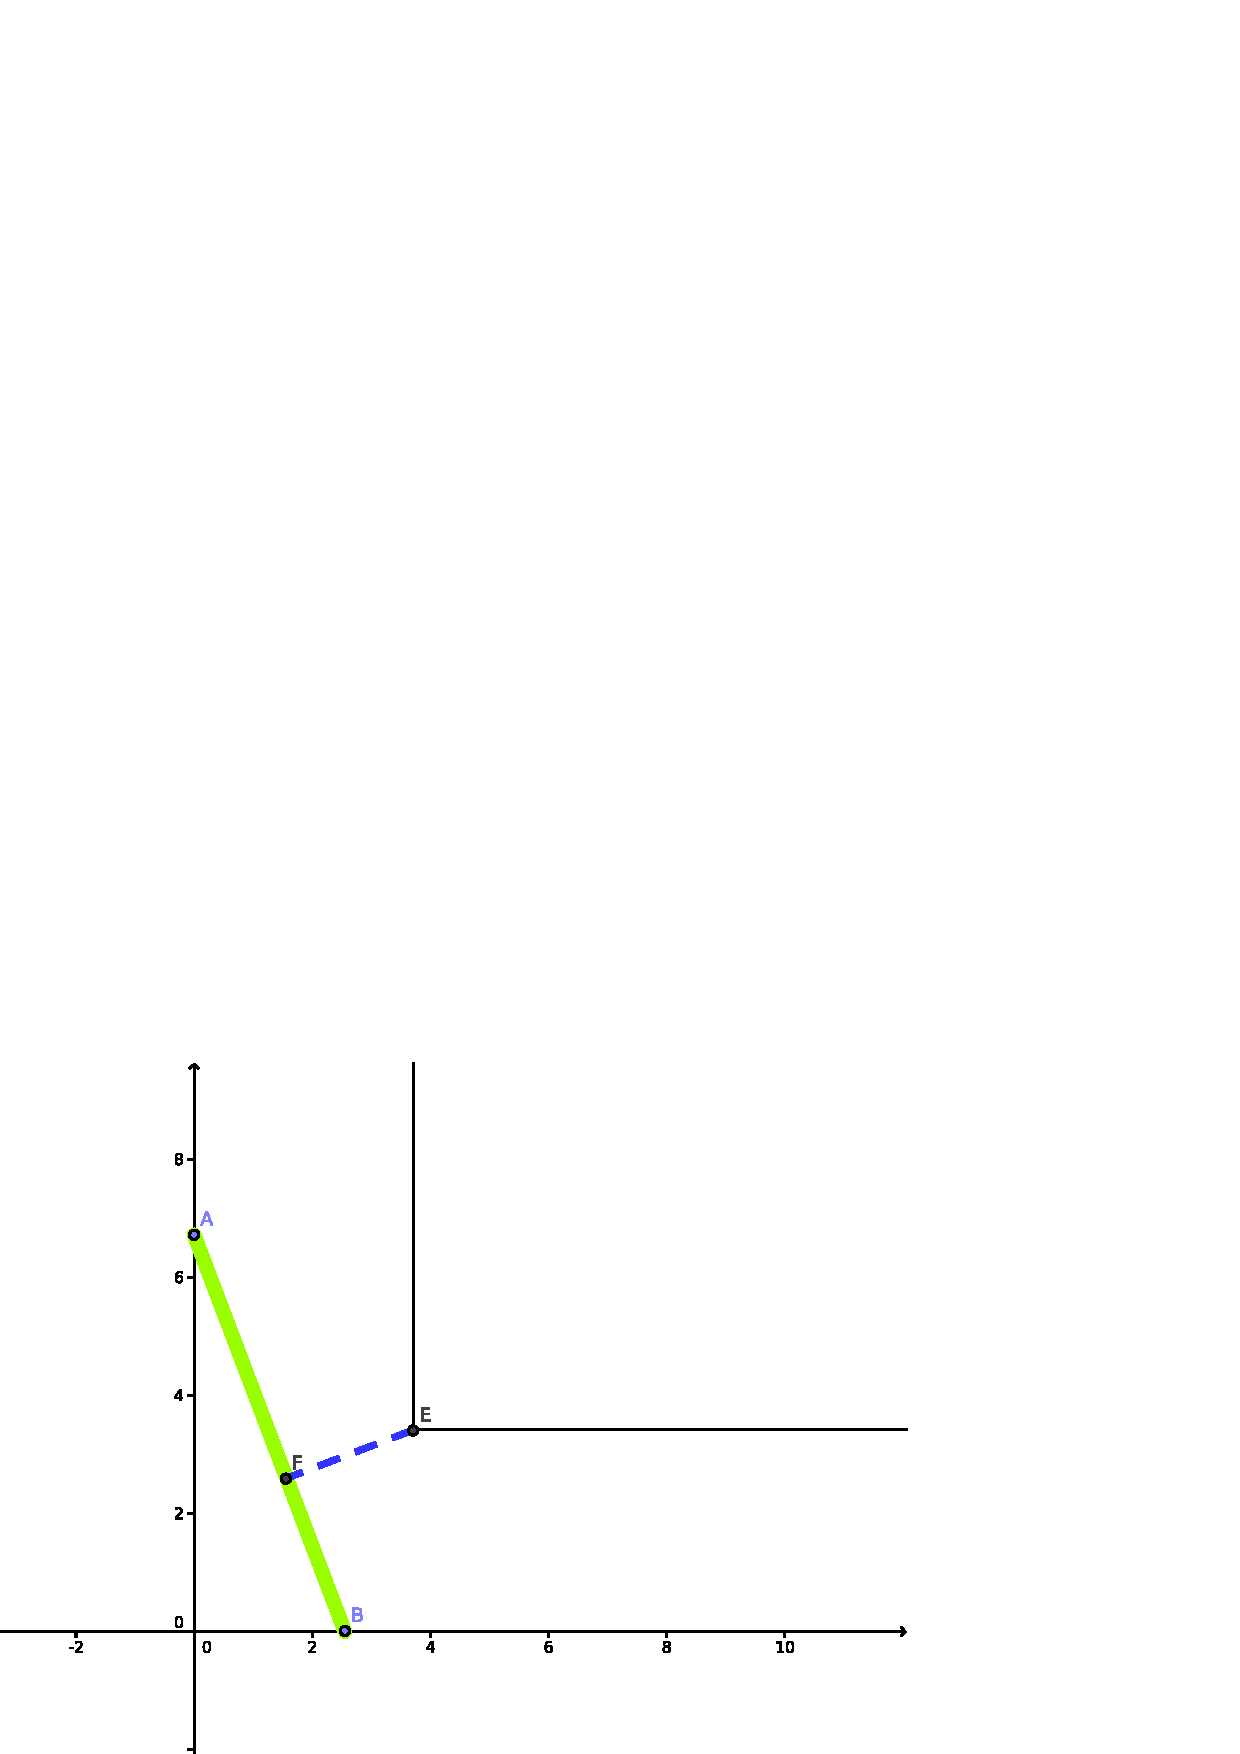
\includegraphics[scale=0.75]{98C.png} } 
	\par
	矮人Greg想要将一个长为$l$宽为$w$的矩形棺材(棺材表面绝对光滑,所以棺材可以任意的滑动)拖过一个L型墓道。如图所示,L型墓道两个走廊的宽度分别是$a$和$b$,呈$90^\circ$,并且走廊的长度远大于$l$。现在矮人Greg想知道对于给定的$a$、$b$、$l$,最大的$w$是多少,或者无论如何也不能通过。

\end{prob}

\begin{sol}
	\begin{center}
		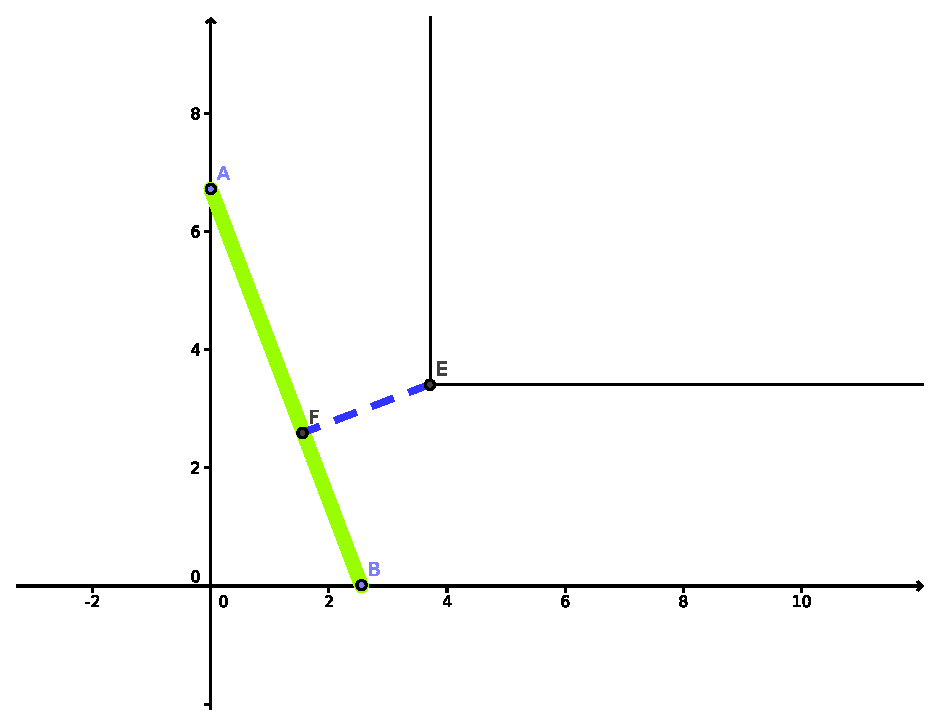
\includegraphics[width=5cm]{98C.eps} 
	\end{center}
	\par
		如图所示,矩形一边沿墙角滑下,可以发现,内拐点到这边的距离是关于时间的单峰函数。三分得到其最小值就是答案。
\end{sol}

\newproblem{191D. Metro Scheme}
\begin{prob}
	给定一个$n$个点$m$条边的仙人掌图(每个点至多属于一个环),可以用链或状将所有边覆盖,且每条边只经过一次。
	求最少需要的链和环的总数。$n \le 10^5, m \le 3 \cdot 10^5$。
\end{prob}

\begin{sol}
	求双连通分量然后dp当然是可以做的,不过非常麻烦。我们不妨考虑原问题的简化版本,
	即原图是树而不是仙人掌。考虑答案最小值,每条路径链接两个奇度数的点。
	于是答案最小值为$\sum_{\forall x \in V}{[d(x)\text{ is odd}]}/2$。这个值实际上是可以达到的,而且随便连只要合法就可以得到这个下界。假设有一条边未被覆盖,那么将这条边断开得到的两个子树中都是偶数个奇度点,算加上这条边就是奇数个奇度点,肯定会一边剩一个奇度点,于是这条边会被覆盖。

	\par
	对于原问题中的环:
	\begin{enumerate}
		\item 环上的点度数都是2,那么ans++;
		\item 环上有一个点度数大于2,同样ans++;
		\item 环上有两个以上的点大于2,这时候可以通过延长这些有外来路径的点来将环完全覆盖,具体的分奇偶度数点来讨论即可。这种情况下答案不变。
	\end{enumerate}
	经过一系列简化后,连双连通都不用求。实现的时候可以将度数为2的环上点一个个删去,不影响答案。

\end{sol}

\newproblem{164D. Minimum Diameter}
\begin{prob}
	给定平面上的$n$个点。你需要去删掉\texttt{恰好}$k$个点$(k<n)$,使得剩下的$n-k$个点所构成的集合的直径尽量小。一个点集的直径是指集合中最远点对的距离。
\end{prob}

\begin{sol}
	如果直接二分答案,只能问题转化为一般图的匹配问题。
	不妨枚举两点作为最远点。设它们的距离为$d$。
	那么形成的两圆之外的点是一定要删除的。
	而在两圆交的部分内的点,需要满足:
	不存在两个点距离大于$d$。
	而交部分的点可以分成两部分,从而变成二分图的匹配问题。
	理论复杂度上限非常高,不过蕴含的常数很小的。
\end{sol}


\section{Volumn VII}
\newproblem{150E. Freezing with Style}
\begin{prob}
	给定一个$n$个点$(n \le 10^5)$,边上带权的树。求一条长度在$l$到$r$之间的路径,使路径上边权的中位数最大。对于一个长度为$m$、下标从0开始的有序数列$a_i$,它的中位数是$a_{\lfloor m/2 \rfloor}$。
\end{prob}

\begin{sol}
	典型的树分治。于是我们只用考虑在一个子树中经过根的路径。首先二分答案(局部二分比全局二分要快)$w$。如果一条边边权大于等于$w$,那么令这条边新的边权为1,否则为0。问题转化成了判断是否存在一条路径上新边权和大于等于0,即求新权值最大的路径。将儿子按其子树深度从大到小排序后,利用单调性这一步可以做到$O(n)$。总复杂度为$O(n \log^2 n)$。
\end{sol}

\newproblem{101E. Candies and Stones}
\begin{prob}
	给定一个$n \times m$的棋盘,每个格子有一个权值。现在要从$(1,1)$走到$(n,m)$,使经过的格子权值总和最大。求方案。要求空间复杂度做到$O(n+m)$。格子的权值以某种压缩的形式给出。$n,m \le 20000$,时限15s。
\end{prob}

\begin{sol}
	如果没有空间限制,那么很容易得到$O(nm)$的dp算法。而如果只算答案,
	用滚动数组也可以优化空间至线性。
	不如将这两者结合起来,考虑运用分治。
	在传统的dp算法中,阶段是按对角线划分的。
	那么对于规模是$n \times m$的棋盘,通过合并前$\frac{n+m}{2}$和后$\frac{n+m}{2}$
	可以得到整个的答案以及第$\frac{n+m}{2}$个阶段上的方案。
	于是可以分成左上和右下两个子矩形递归下去做。\par
	复杂度分析:每次矩形的规模$n \times m$至少缩小至$nm/4$。
	所以$T(nm) = O(nm) + 2T(nm/4) = O(nm)$。
\end{sol}

\newproblem{103E. Buying Sets}
\begin{prob}
	给定$n$个集合,每个集合包含若干个$1$到$n$的整数,另外还有一个整数权值。保证任意$k$个集合的并的元素个数不小于$k$。求一个集合的集合,使得集合的集合的大小等于所选集合并的元素个数,且权值和最大。$n \le 300$。
\end{prob}

\begin{sol}
	首先建立二分图,左边对应集合,右边对应数。如果第$i$个集合包含数$j$,那么连有向边$u_i \to v_j$($u$是左边点,$v$对应右边点)。由Hall定理,以及题目的特殊性,该二分图有完备匹配。求出这个完备匹配。这样以来相当于给每个数找了一个配对的集合。
	然后,将左边的点和右边的点按完备匹配合并成一个点,保留对应的边,得到一个DAG。可以发现,任何一个合法的解在DAG中都不存在出边,反过来也成立。于是问题转化为最大权闭合子图,可以用最大流最小割模型解决。
\end{sol}

\newproblem{105E. Lift and Throw}
\begin{prob}
	三个人初始时站在数轴整点上。任意一个人可以进行以下操作不超过一次:
	\begin{enumerate}
		\item 移动一段距离,不超过一个定值。
		\item 抓起另一个人,要求两人距离恰好为1。一但抓起一个人后,将不能移动。被抓起的人不能进行任何操作。
		\item 将抓起的人扔一段距离,不超过一个定值。
	\end{enumerate}
	求三人中任意一人能到达的最远距离。输入所有数均为整数且不超过10。
\end{prob}

\begin{sol}
	爆搜+记忆化剪枝,over。
\end{sol}

\newproblem{107D. Crime Management}
\begin{prob}
	构造一个长度为$n$的字符串,由大写字母组成。
	对于每个字母有个系数$c_i$,要求$i$字母
	出现次数为$c_i$的倍数。满足所有$c$的最小
	公倍数不超过$123$。求合法构造方案数模$12345$。
\end{prob}

\begin{sol}
	由于所有$c$的最小公倍数不超过123,可能的状态总数也不超过123。dfs预处理出所有状态以及相互的转移,最后用矩阵快速幂加速。
\end{sol}

\newproblem{113D. Museum}
\begin{prob}
	有一个$n(n \le 22)$个点的无向图。一开始Alice和Bob分别站在$a$,$b$点。每一回合,Alice和Bob将等概率随机走向某个相邻点。求对于每个点Alice和Bob在此相遇的概率。注意:一但相遇则停止游戏。
\end{prob}

\begin{sol}
	按照常规思路,未知量用二维信息来表示,可以得到$O(n^2)$个变量的方程组。用高斯消元一次是$O(n^6)$,做$n$次将达到$O(n^7)$,无法承受。\par
	原来计算的是$Ax = b$,其中只有$A$是$n^2 \times n^2$的矩阵,而$b$是$n^2 \times 1$的向量。实际上每次换一个终点计算,仅仅改变了$b$。那么可以将$b$换成$n^2 \times n$的矩阵,一次消元就能算出所有解。于是复杂度变为了$O(n^6)$。
\end{sol}

\newproblem{115D. Unambiguous Arithmetic Expression}
\begin{prob}
	定义UAE为:
	\begin{enumerate}
		\item 单独一个非负整数是UAE。
		\item 如果$X$和$Y$是两个UAE,那么
			$(X)+(Y)$,$(X)-(Y)$,$(X)*(Y)$,$(X)/(Y)$都是UAE。
		\item 如果$X$是UAE,那么$-(X)$和$+(X)$也是。
	\end{enumerate}
	给定一个仅包含数字和+-*/的字符串,求添加任意对括号后能形成的合法UAE数目。
	长度不超过2000。
\end{prob}

\begin{sol}
	因为第三个限制,可以考虑从右到左进行构造。\par
	令$f[i][j]$表示进行到了第$i$个字符,第$i$个字符之后
	是$j$个块相加的形式(因为一旦套上括号后就跟数字无异了)。
	为了方便处理,将所有数字替换为a。
	如果$i-1$是a,那么显然$i-1$和$i$要按第二个规则构造。
	转移到$f[i-2][k], \forall 1 \le k \le j+1$。
	否则,如果$i$是+-,那么按第三个规则构造,转移到
	$f[i-1][k], \forall 1 \le k \le j$。答案就是$f[0][1]$。
	\par 这样的复杂度是$O(n^3)$。通过部分和优化可以做到$O(n^2)$。
\end{sol}

\newproblem{120I. Luck is in Numbers}
\begin{prob}
	对于一个位数为偶数的数字,将它从中间切开,分成长度相同的两部分。
	然后重叠在一起。那么交的个数称为这个数字的幸运度。\par
	给定一个$k(k \le 2 \times 10^5)$位数,求位数相同且大于这个数,同时幸运度也更大的最小的数。
\end{prob}

\begin{sol}
	主要思路是贪心。预处理出任意两数码交的个数。注意到8这个数字非常imba。
	从高位到低位处理,改变当前位,之后全部填8,看是否满足条件。如果满足就确定这一位。否则无解。通过部分和预处理可以使验证是$O(1)$的。总复杂度为$O(10k)$。
\end{sol}

\newproblem{123E. Maze}
\begin{prob}
	一个maze由一个树表示。考虑一个如下的子过程:
	\begin{verbatim}
	    DFS(x)
	        if x == exit vertex then
	            finish search
	        flag[x] <- TRUE
	        random shuffle the vertices' order in V(x) 
	        for i <- 1 to length[V] do
	            if flag[V[i]] = FALSE then
	                count++;
	                DFS(y);
	        count++;
	\end{verbatim} 
	\par
	现在给出每个点选为起点和终点的概率,求\verb#count#的期望值。
	点数不超过$10^5$。
\end{prob}

\begin{sol}
	设起点为$s$,终点为$t$,$s$到$t$路径上点数为$l$。
	如果以$s$为根建树,$sz[x]$表示$x$的子树大小(不含$x$)。
	那么$t$子树中的点一定不会被经过。
	而$s->t$对答案的贡献为$l-1$。称$s->t$为主轴,那么
	父亲在主轴上,本身又不在主轴上的点所代表的子树对
	答案的贡献又是什么呢? \par
	注意到,一旦偏离主轴进入某个点$u$,那么一定是$u$子树
	中所有点都要走遍,这些点对答案的贡献是2(一进一出)。
	设$u$的父亲是$p$,$p$主轴上的儿子是$v$。进入$u$的概率等于$p$儿子的所有排列中
	$u$在$v$前面的概率,即$\frac{1}{2}$。于是,
	每个不在主轴上且不在$t$子树中的点对答案的贡献恰好是1。
	设总点数为$n$。那么以$s$为起点,$t$为终点的期望答案
	就是$n-l-sz[t]+l-1 = n-sz[t]-1$,只与$t$的子树大小有关。
	于是乎,在一遍dfs过程中动态修改根,维护所有点sz与作为终点概率的乘积和即可。
\end{sol}

\newproblem{125E. MST Company}
\begin{prob}
	求满足度限制的最小生成树。即要求某个点$u$的度恰好为$k$。
	点数$n \le 5000$,边数$m \le 10^5$,$k \le 5000$。
\end{prob}

\begin{sol}
	传统最小度限制生成树的做法基于贪心:先将$u$删掉,用kruskal求最小生成森林。
	再考虑将与$u$关联的边往上加。如果加上去形成环,
	就置换掉最大的边(如果可以使答案变小的话)。复杂度是$O(m\log m + nk)$。
	\par 还有一种基于实数二分的方法。将所有与$u$关联的边加上一个实数$w$。
	令$f(w)$表示加上$w$后与$u$关联的边在最小生成树中的条数。
	显然,$f(w)$是单调不增函数。当$f(w) = k$时,新图的最小生成树就是答案。
	反证很容易证明。复杂度为$O(m \log m \log w)$,与$k$无关。
\end{sol}


\section{Volumn VIII}
\newproblem{193E. Fibonacci Number}
\begin{prob}
	考虑fibonacci数列每项模$10^{13}$后得到的数列。问$x$在这个数列中是
	否出现过,如果出现过,求最早出现位置。
\end{prob}

\begin{sol}
	如果$x$模$10^i$为$d$,那么$x$模$10^{i+1}$的结果必然是
	以$d$为后缀的。于是基本思路就是由模$10^i$的
	答案列表推出模$10^{i+1}$的答案列表,最后得到模$10^{13}$的答案。
	
	\par 将$10^i$推到$10^{i+1}$时,需要将列表按循环节长度
	平铺多次,再通过矩阵乘法快速幂验证。因此,我们需要知道
	fibonacci数列模$n$的循环节,设为$L(n)$。这里有一个定理:\par
	设$n$的质因数分解为$n = p_1^{m_1} p_2^{m_2} \ldots p_k^{m_k}$,
	那么$L(n)=lcm(L(p_1^{m_1}), L(p_2^{m_2}), \ldots)$,
	$L(p_i^{m_i}) = L(p_i)p_i^{m_{i}-1}$。
	\par
	为了避免边界情况,先暴力构造出$10^3$的列表。注意到$L(10^k)=10L(10^k-1), k \ge 4$,
	那么每次平铺10次,然后验证即可。复杂度比较诡异,实测非常快。
\end{sol}

\newproblem{145D. Lucky Pair}
\begin{prob}
	幸运数字是那些仅由$4$和$7$构成的数字。
	有一个长度为$n$的非负整数序列$A$,要从整个序列中选出两个互
	不相交的子段$A[l_1,r_1], A[l_2,r_2] (1 \le l_1 \le r_1 < l_2 \le r_2 \le n)$
	,使得不存在某个幸运数字既在$A[l_1,r_1]$出现,又在$A[l_2,r_2]$出现。求有多少种
	选择方案。保证$A$序列中幸运数字的总出现次数不会超过$1000$次。$n \le 10^5$。
\end{prob}

\begin{sol}
	注意到非幸运数字都是等价的,可以先把幸运数字找出来。
	设$X[i]$为从左数第$i$个幸运数字。再将非幸运数字合并到一块。
	\par 因为幸运数字不是很多,可以枚举左区间。
	具体的,先枚举左区间最靠右的幸运数字是第$r$个。
	然后从左往右枚举左区间最靠左的是第$l$个。
	注意到一旦$X[l]$在$X[l+1] \ldots X[r]$不再出现,
	那么右区间就可以包含这个数了。于是用并差集维护
	所有极大合法右区间,其任意子区间都合法。一旦一个
	新的幸运数字变为合法,那么合并两个极大合法右区间。
	算法复杂度为$O(k^2)$,$k$是幸运数字个数。\par
	需要注意的是,实现上细节很多。问题主要在左右区间交界
	处,需要仔细斟酌,耐心编码。
\end{sol}

\newproblem{132E. Bits of merry old England}
\begin{prob}
	你被要求输出一个由$n$个数$(n\le 250)$组成的序列。有$m$个
	变量$(m\le 26)$给你用,变量必须是单个小写英文字母 \par。
	要求给出一个操作序列,输出这$n$个数。操作只有2种:
	\begin{enumerate}
		\item 对某个变量赋值,代价为该值二进制表示中1的个数。
		\item 输出某个变量,无代价。
	\end{enumerate}
	变量没有初值,也就是,你必须给变量赋过值才能输出这个变量。
	要求最小化操作序列的代价。 输出这个最小代价,以及能达到最小代价的满足条件的操作序列。
\end{prob}

\begin{sol}
	首先可以确定需要用多少个变量。设$n$个数中不同的数的个数为$z$。
	那么\textbf{恰好}需要$t = \min \{ m, z\}$个变量。
	建一个$n+t$个点边带权的DAG。前$n$个点对应序列中的数。
	从第$i$个点向第$j$个点连边$(i < j \le n)$。边权的话,如果序列中
	$i,j$位置的值相同,那么为0。否则为$j$二进制表示中1的个数。
	对于附加的$t$个点,从第$n+i$向$j$连边$(j \le n)$,权值为
	$j$二进制表示中1的个数。于是乎,这个DAG的最小路径覆盖数
	恰好为$t$。最小路径覆盖可以由二分图匹配解决。那么既然
	控制了匹配数,求出的最佳匹配(或最小费用流)就是满足最小代价
	的方案。
\end{sol}

\newproblem{138D. World of Darkraft}
\begin{prob}
	给定一个$n \times m (n,m \le 20)$的棋盘。棋盘上有3类格子(L,R,X)。
	两个人轮流进行游戏。每轮每人选择一个未被标记的格子。
	根据不同格子触发相应的效果:
	\begin{itemize}
		\item L --- 从这个格子出发往左下和右上方向走,每
			遇到一个未被标记的格子则标记之,
			直到遇到一个已标记的格子或者超出棋盘边界。
		\item R --- 与L类似,唯一差别在于扩展方向是左上
			和右下。
		\item X --- 结合L和R的效果。
	\end{itemize}
	不能移动者输。问是否先手必胜。
\end{prob}

\begin{sol}
	由于所有操作都是斜对角线上,可以将棋盘黑白染色单独处理,
	最后通过求独立游戏的和(即异或)来得到整个游戏的答案。
	\par
	然后将棋盘转$45^{\circ}$。每次操作变成在行和列上进行。
	而每次操作会划分成若干个子棋盘,互为独立游戏。
	于是可以动态规划来求出sg函数的值。状态记录当前矩形。
	复杂度是$O(n^4m^4)$。
\end{sol}

\newproblem{140F. New Year Snowflake}
\begin{prob}
	一个点集是中心对称的,指存在一
	个点$X$(不一定要属于这个点集),对
	于任意点集中一点$a$,一定有
	点集中某点$b$($b$可以和$a$相同),使得
	$b$是$a$关于$X$的对称点。此时
	称$X$为点集的对称中心。\par 现给定平面内$n$个点的集合,
	你可以添加最多$m$个点(也可以
	不添加),使得添加后的点集是中心对称的。问有多少个不同的点可能成为对
	称中心,并将他们的坐标输出。
	如果可能有无穷多个对称中心,输出$-1$。$n \le 2 \times 10^4, m \le 10$。
\end{prob}

\begin{sol}
	显然,如果$n \le m$,那么输出-1。\par
	否则,只要能确定所有可能的对称中心,就可以$O(n)$用Hash验证了。
	\par 将所有点按x坐标排序。那么可能的对称中心只可能是
	前$m+1$个点与后$m+1$个点自由组合得到的$(m+1)^2$个中点。
	因为即便添加$m$个x坐标极小的点,第$m+1$个点也能与倒数第$m+1$个点配对。
	否则会与后$m$个点配对。倒数第$m+1$个点同理。于是便解决了。
\end{sol}

\newproblem{147B. Smile House}
\begin{prob}
	给出一个$n(n \le 150)$个点边上带权的有向图。
	求正权环(环上路径和为正)的最小长度。
\end{prob}

\begin{sol}
	修改矩阵乘法,原来是:
	\begin{displaymath}
		c[i][j] = \sum a[i][k] \times b[k][j]
	\end{displaymath}
	修改为:
	\begin{displaymath}
		c[i][j] = \max \{a[i][k] + b[k][j]\}
	\end{displaymath}
	可以验证修改后的矩阵乘法依然满足结合律。于是
	也能进行快速幂。(类似与$O(n^3 \log n)$的APSP最短路)\par
	现在简化问题。设$E$是边权的邻接矩阵。
	我们要求的是最小的$t$,满足$F=E^t$中存在$k$,$F[k][k] > 0$。
	运用倍增即可求出。(类似倍增LCA)。复杂度为$O(n^3 \log n)$。
\end{sol}

\newproblem{152D. Frame}
\begin{prob}
	在一个$n \times m$的棋盘上画两个矩形边框,
	可以任意重叠,甚至重合。现在给你最终的图案,
	问是否可能通过这样画两个矩形边框的方式
	得到。$n, m \le 1000$。
\end{prob}

\begin{sol}
	如果一行或者一列有超过3个连续的\#,那么必然
	是一个矩形的边界。确定两个矩形边界后,可以
	$O(n)$验证。\par
	除了一个例外情况:一个矩形的长或宽为3。不难
	发现,这种情况下,边界一定是在最大(小),
	次大(次小)上。单独处理即可。
\end{sol}

\newproblem{183D. T-shirt}
\begin{prob}
	有$n$个人,$m$种衬衫尺寸。你要带$n$件衣服分配到每个人
	身上。但是你只知道第$i$个人穿$j$尺寸衬衫的概率是$p[i][j]$。
	求一种方案,使期望配对上的衬衫数目最大。
\end{prob}

\begin{sol}
	由于衬衫尺寸之间是独立的,我们可以先计算这样一个数组。
	定义$f[i][j][k]$表示对于$i$尺寸,前$j$个人中至少$k$
	个人是这个尺寸的概率。转移:
	\begin{displaymath}
		f[i][j][k] = (1-p[j][i]) \times f[i][j-1][k] 
		+ p[j][i] \times f[i][j-1][k-1]
	\end{displaymath}
	答案可以贪心得到,即$f$数组中最大的$n$项对应的期望。
	不过这样的复杂度会达到$O(n^2m)$,无法承受。\par
	注意到只需求出最大的$n$项,可以先对于所有$i,k$,求
	出$f[i][1][k]$。因为$f[i][j][k] \le f[i][j][k-1]$,
	所以每次只需选出当前最大的$i$,然后扩展出下一项。
	扩展过程可以做到$O(n)$。因为:
	\begin{eqnarray}
		f[i][j][k] &=&(1-p[j][i]) \times f[i][j-1][k] \nonumber \\
					&+& p[j][i] \times f[i][j-1][k-1]\text{(已知)\nonumber}
	\end{eqnarray}
	,而:
	\begin{eqnarray}
		f[i][j-1][k] &=& (1-p[j-1][i]) \times f[i][j-2][k] \nonumber \\
					&+& p[j-1][i] \times f[i][j-2][k-1]\text{(已知)} \nonumber 
	\end{eqnarray}
	如此下去,未被计算的只有$O(n)$个状态。于是这样下来,
	总复杂度为$O(n^2)$。
\end{sol}

\newproblem{217E. Alien DNA}
\begin{prob}
	给出一段仅有A,C,G,T组成的长为$n(n \le 3 \times 10^6)$
	的字符串$s$。
	一次操作指给出区间$[l,r](l,r \le 10^9)$,然后在$r$之后插入
	交替变换组成的长为$r-l+1$的字符串:
	$s_{l+1}s_{l+3}\cdots s_{l}s_{l+2}\cdots$。
	\par
	现在给出所有操作(总数不超过$5000$),
	求最终序列的前$k(k \le 3 \times 10^6)$个字符。
\end{prob}

\begin{sol}
	倒着考虑原问题。可以确定最后一次操作
	的位置是$[l,r]$,产生的是$[r+1,r+r-l+1]$这一段。
	那么可以将$[r+1,r+r-l+1]$截去,得到不包含
	最后一次操作的序列。于是可以递归做下去。\par
	然后考虑用数据结构来维护。
	偷懒的办法是用STL中的rope,支持string
	支持的所有操作,且复杂度为根号级别。

\end{sol}

\newproblem{135E. Weak Subsequence}
\begin{prob}
	对于一个字符集大小为$k$的字符串$s$,如果称它是合法的
	要求其中最长的子串同时也是$s$的弱子序列的长度为$w$。
	\par
	如果说长为$n$的字符串$a$是长为$m$的字符串$b$的弱子序列,
	只存在$1 \le i_1 < i_2 < \cdots < i_n \le m$,且:
	\begin{itemize}
		\item $\forall 1 \le k \le n, a_k = S_{i_k}$;
		\item $\exists k, i_{k+1} - i_k > 1$。
	\end{itemize}
	求合法字符串的个数模$10^9+7$。$k \le 10^6, w \le 10^9$。
\end{prob}

\begin{sol}
	弱子序列的定义比较奇怪,可以从这里入手。
	容易发现,强化其定义,即设从$l$到$r$的子串
	是原串的弱子序列,等价与存在$k > r$,且$s[k] = s[r]$,
	或者存在$k < l$,且$s[k] = s[l]$。这样以来只与$l$和$r$
	中的一个有关了。即,为原串的前缀或后缀,且前缀(以前缀为例)
	的最后一个元素在之后还有出现。\par
	进一步放宽限制,最长合法前缀的长度不超过$t$等价
	于字符串后$n-t$($n$为长度)个元素互不相同。设计函数
	$f(n,a,b)$为长度是$n$,前$a$个字符互不相同,后
	$b$个字符互不相同的字符串个数。$f(n,a,b)$很容易通过
	组合基本知识预处理后在$O(1)$求出。于是,枚举长度$n$,
	答案为$f(n,n-w,n-w)-f(n,n-(w-1),n-(w-1))$。这种
	放宽限制的思想没有任何特殊情况需要考虑,
	实在巧妙。
\end{sol}


\section{Volume IX}
\newproblem{163D. Large Refrigerator}
\begin{prob}
	对于确定体积的长方体,求其中表面积最小的三边长。
	体积$V \le 10^{18}$,以质因数分解的形式给出。
\end{prob}

\begin{sol}
	设所求长方体三边长为$a,b,c,a \le b \le c$。首先
	枚举$a$的取值。问题变成了对于$V/a$,求$b,c$,
	满足$bc = V/a$且$b+c$最小。这里可以对$V/a$记忆化
	剪枝。最优化剪枝即当$b=c$时可以取得$b+c$的最小值,
	如果仍然大于当前答案,则没必要继续下去。
	枚举$a$最好从大到小枚举,便于最优化剪枝。
	然后差不多就可以过了。
\end{sol}

\newproblem{167E. Wizards and Bets}
\begin{prob}
	有一个$n$个点$m$条边的DAG。没有入边的点为源,
	没有出边的点为汇,保证源和汇的数目是相同的。
	现在要从图中选出$k$条路径,分别从某个源出发到达某个汇。
	每个源汇都恰被一条路径覆盖一次,任何路径不在
	顶点处相交。\par
	假设终止于$i$号汇的路径是由源$a_i$出发的,我
	们称汇对$(i,j)$是一个逆序对当且仅当$i<j$且$a_i>a_j$
	。如果所有汇对$(i,j)$ $(1 \le i<j \le k)$中的逆序对
	总数是偶数,那么计数器加1,否则减1。\par
	现在,对于所有合法的路径集合,都要对计数器产生影响。
	问最后计数器的值是多少。$n \le 600, m \le 10^5$。
\end{prob}

\begin{sol}
	首先要对“任何路径不相交”下手。假设$u \to p$,$v \to q$
	两条路径于$t$点相交,那么更改$u \to p = u \to t + t \to q$,
	$v \to q = v \to t + t \to p$,这两种情况奇偶性不同对答案的贡献
	恰好为0。因此这个条件可以直接无视。
	\par 
	dp预处理出从任意一个源到任意一个汇的方案数。于是最终答案为:
	\begin{displaymath}
		\sum_{g \in \text{all permutation}} sgn(g) \cdot 
		\prod_{1 \le i \le n} f[i][g[i]]
	\end{displaymath}
	其中,$g$是枚举所有配对方案,$sgn(g)$是$g$中逆序对数的奇偶性
	对应的权值($+-1$),后面的乘积是情况数。\par
	可以发现,这个式子就等于$f$的行列式。\par
	行列式$O(n^3)$的求法:将行列式当成矩阵进行
	高斯消元。交换两行对应行列式取倒数。将
	某行乘上一个系数对应行列式乘同样的系数。
	行与行之间做减法行列式不变。最后消成上
	三角矩阵。而三角矩阵行列式为对角线乘积。
\end{sol}

\newproblem{232D. Fence}
\begin{prob}
	给定一个序列$a_1,a_2,\cdots,a_n$
	以及$q$个询问$(l_1,r_1),(l_2,r_2),\cdots,(l_q,r_q)$。
	对于每个询问$(l_i,r_i)$,回答$(l_j,r_j)$二元组的个数
	,满足$r_j-l_j+1=r_i-l_i+1$,
	且$[l_j,r_j] \cap [l_i,r_i] = \varnothing$,且
	对于所有$0 \le k \le r_i-l_i$,
	使$a[l_i+k]+a[l_j+k]=a[l_i]+a[l_j]$。
	$n \le 10^5$。
\end{prob}

\begin{sol}
	先将原序列相邻两项做差得到长度为
	$n-1$的$b$序列,就变成了询问一段
	取反后相同的且不交的段数。构造一
	个$s$序列为$b\$-b$,然后就变成了
	经典的后缀数组离线询问的问题了。
	复杂度为$O(n \log n+q\log n)$。
\end{sol}

\newproblem{175E. Power Defence}
\begin{prob}
	在一个塔防游戏中,boss从x轴的
	负无穷走到正无穷,可以在$y=1$和$y=-1$
	两条直线上的整点处建三种塔:火、电、冰。每种
	塔有一个攻击半径和每秒伤害(除冰塔外)。
	在某一时刻,boss走到$k$个冰塔的攻击半径内
	,则移动速度减为原来的$1/(k+1)$。给定每种
	塔的总数$(\le 20)$,求最大化伤害的方案。
\end{prob}

\begin{sol}
	首先,可以把$y=-1$的塔对称到$y=1$
	上,问题变成了在$y=1$上每个整点可以
	修不超过2个塔。可以发现,塔必然是连续
	的一段,且不能有相邻位置都只有1个塔
	,所以可以暴力出冰塔的修建方案。之后
	进行dp:用$f[i][j][k]$表示在前$i$个
	位置修了$j$个火,$k$个电塔,$O(1)$转移。
	\par 优化:所有塔肯定必须用,塔连续一段的
	长度$\le 13$(实际上10就够了)。
\end{sol}

\newproblem{176D. Hyper string}
\begin{prob}
	计算一个Hyper string和一个长度不超过2000且仅
	由小写字母构成的字符串的最长公共子序列。
	Hyper string是由多个基本字符串连接而成的。每个
	基本字符串长度不超过$2000$,且长度之和不超过$10^6$。
\end{prob}

\begin{sol}
	首先考虑一个简化版问题:计算一个长度
	不超过2000的字符串$s_1$和一个长度不超过$10^6$的
	字符串$s_2$的LCS。传统的dp方法复杂度将达到$O(n^2)$,
	不能承受。注意到题目特殊性,答案不是很大,且
	仅由26个小写字母构成。
	可以换一种状态定义方式。定义$f[i][j]$表示$s_1$
	进行到$i$,答案为$j$,在$s_2$中最靠前的位置。
	转移只需看$s_1[i+1]$在$s_2[f[i][j]]$之后第
	一次出现的位置。预处理出$s_2$中每个位置
	之后第一个出现每个字母的位置,可以使复杂度
	做到$O(n^2)$。\par
	回到原问题,不难发现本质做法一样。唯一区别
	在于$f[i][j]$记录两个东西,一个是基本字符串编号,
	一个是在基本字符串中的位置。转移类似,预处理也类似,
	复杂度也是$O(n^2)$。
\end{sol}

\newproblem{178F. Representative Sampling}
\begin{prob}
	有$n(n \le 2000)$个由26个小写字母组成的字符串,要求从中
	选出$k$个,使该集合的权值最大。设$S$为
	选择的集合,则权值定义如下:
	\begin{displaymath}
		\sum_{i,j \in S} \text{$i$,$j$最长公共前缀的长度}
	\end{displaymath}
\end{prob}

\begin{sol}
	初一看,很容易想到用trie这种前缀处理工具。
	将所有字符串插入trie中后,变成了标记$k$个点,
	每个点的权值定义为$m(m-1)$,$m$是子树中标记点
	的数目。于是可以设计一个状态$O(n^2)$,转移$O(n)$
	的树型dp,总复杂度为$O(n^3)$。走到这里就难以
	继续走下去。只好另辟蹊径。\par
	联想到后缀数组求lcp的方法,可以
	将所有字符串按字典序排序。设计状态$f[l][r][k]$
	表示区间$[l,r]$选$k$个的答案。于是:
	\begin{displaymath}
		f[l][r][k] = \max_{l \le  t \le k}\{ f[l][p][t] + f[p+1][r][k-t] + \text{something}\}
	\end{displaymath}
	注意到$p$取值的随意性,不妨取相邻两字符串LCP最小的那个位置。于是:
	\begin{displaymath}
	f[l][r][k] = \max_{l \le  t \le k}\{ f[l][p][t] + f[p+1][r][k-t] + t(k-t) \cdot lcp[p]\}
\end{displaymath}
有用的区间只有$O(n)$个。复杂度比较难算,考虑两类极端情况:
$p=l+1$,转移是$O(1)$的,总共是$O(n^2)$;
$p=(l+r)/2$,$T(n) = (n/2)^2 + 2T(n/2) = O(n^2 \log n)$。
是一个十分优秀的算法。
\end{sol}

\newproblem{178E. The Beaver's Problem II}
\begin{prob}
	给出一个黑白图片$(2000 \times 2000)$,里面
	仅包含正方形和圆,可能经过任意次旋转。
	每个像素有$20\%$概率反色。统计正方形和
	圆的数目。
\end{prob}

\begin{sol}
	这是一道非常偏向实际应用的图像处理题。
	整个算法分两步:噪音消除和模糊统计。\par
	噪音消除的方法:对于每个像素,如果四周有
	白色像素,那么在新图中为白色,否则为黑色。
	然后再对新图黑白颠倒做一遍。剩下的图形
	噪音就不是很多了。\par
	然后bfs出所有黑色连通块。如果大小太小说明是
	噪音,直接删掉。否则判断是正方形还是圆。\par
	这可以利用圆和正方形的差异来解决。首先
	算出中心,用平均坐标即可。然后计算半径,
	即离中心最远点距离,设为$r$。对于圆来说,
	落在$\frac{\sqrt{2}}{2} r - r$的点数接近
	总点数的一半,而正方形则很少。就可以通过
	CF上的数据了。
\end{sol}

\newproblem{180B. Divisibility Rules}
\begin{prob}
	如果检查一个数能否被2,4,5,8,10整除的时候只需要检查它的最后一位或几位是否满足某个条件。这种规则称为2类型规则(2-type)。\par
	如果检查一个数能否被给定的数整除意味着计算这个数的各个数位上的数字之和并判断这个和能否被给定的数整除,那么称这个规则为3类型规则(3-type)。\par
	如果我们需要求出一个数的奇数位上的数字之和与偶数位上的数字之和的差值去检查这个差值能否被给定数整除,那么这个规则被称为11类型规则(11-type)。\par
	有些情况下我们应当把除数分解成一些因数然后检查是否满足一些不同类型的规则(2-type,3-type,11-type)。这样混合的整除规则被称为6类型规则(6-type)。 \par
	最后,有些除数是所有类型的规则都无效的,称在这种情况下神秘的7类型规则(7-type)有效。\par
	要求出$b$进制下除数为$d$的整除规则类型。$b,d \le 100$。
\end{prob}

\begin{sol}
	将一个数$x$写成$b^0 d_0 + b^1 d_1 + b^2 d_2 \cdots$的形式。
	对于每种类型分别讨论:
	\begin{enumerate}
		\item 2-type: 意味着$\exists k, b^k = b^{k+1} = \cdots \equiv 0 \pmod d$。
			通过不断乘$b$知道能被$d$整除来判断。
		\item 3-type: 意味着$\forall i, b^i \equiv 1 \pmod d$,即$b \equiv 1 \pmod d$。
		\item 11-type: 意味着$\forall i, b^{2i} \equiv 1 \pmod d, b^{2i+1} \equiv -1 \pmod d$,
			或者反过来。即$b \equiv -1 \pmod d$。
		\item 6-type: 分解开,然后判断。
	\end{enumerate}
\end{sol}

\newproblem{185D. Visit of the Great}
\begin{prob}
	给出$l,r,p(l,r \le 10^{18}, p \le 10^9)$,计算$lcm(k^{2^l}+1, k^{2^{l+1}}, 
	\cdots, k^{2^r}+1) \mod p$,$p$是质数。$10^5$组数据。
\end{prob}

\begin{sol}
	首先尝试简化$lcm$。可以发现,$gcd(k^{2^i}+1, k^{2^{j}}+1)
	= gcd(k^{2^i}+1, 2)$。于是若$k$是奇数,那么所有
	数都含2这个质因子,且公共的质因子仅有2;若是偶数,那么
	两两互质。考虑偶数情况:
	\begin{eqnarray}
		lcm & = & (k^{2^l}+1) \cdot (k^{2^{l+1}}+1) \cdots (k^{2^r}+1) \\
			& = & \frac{k^{2^{r+1}}-1}{k^{2^{l}}-1} \\
		   & = & (k^{2^l}+1) \cdot (k^{2^{l+1}}+1) \cdots (k^{2^r}+1)
	\end{eqnarray}
	如果$(2)$中分母模$p$为0,那么通过$(3)$式可以得到答案为$2^{r-l} \mod p$,
	否则直接逆元。奇数情况类似,不再赘述。
\end{sol}

\newproblem{187D. BRT Contract}
\begin{prob}
	一条路上有$n$个红绿灯,共$n+1$段路。
	起点为左端点,终点为右端点。给出每段路的长度。
	已知所有红绿灯的绿灯周期均为$g$,
	红灯周期均为$r$,且在$[0, g)$时刻(模$g+r$意义下)区间内为绿灯,
	$[g, g+r)$时刻区间内为红灯。\par
	现在有$q$辆公交车从起点出发,开向终点,
	第$i$辆公交出发时刻为$t_i$。求所有公交
	到达终点的时刻。$n \le 10^5$。
\end{prob}

\begin{sol}
	可以发现,一旦公交停在某个红绿灯前,
	下一次出发又是从$0$时刻开始。因此,
	可以预处理一个数组$f$,其中$f[i]$
	表示$0$时刻在第$i$个红绿灯前,到达终点
	的时刻。这个可以通过递推来得到。假设
	已经算出了$k+1 \cdots n$的$f$值。在
	计算$f[k]$时,只需知道从$k$出发第一个
	遇到的红灯是第$t$个,那么$f[k]=$$k$到
	$t$距离$+$等待时间$+f[t]$。利用
	前缀和可以算出从$k$到之后任意位置不停留
	的路程,找到最靠左的落在$[g,g+r)$区间内
	就是停靠的红绿灯。这可以用线段树来实现。
	\par 对于从起点出发的公交车处理方法是
	一样的,同样只需找到第一个停靠位置就能
	推出答案了。
\end{sol}


\section{Volume X}
\newproblem{176E. Archaeology}
\begin{prob}
	给出一棵$n(n \le 10^5)$个节点,边带权的树。
	节点有黑白两色。一开始所有点都是白色。
	有$q(q \le 10^5)$个操作,共三种形式:
	\begin{enumerate}
		\item 将一个节点染为黑色
		\item 将一个节点染为白色
		\item 询问使所有黑色节点两两互达的
			最小权边集是多少。
	\end{enumerate}
\end{prob}

\begin{sol}
	显然,答案就是两两黑色节点之间
	路径的并。我们需要找一个统计方法,
	满足并中每条边都被算到恰好一次,且
	不在并中的边都不被算到。\par
	将黑色节点按照dfs序排序。那么答案就是
	每个黑点到它和它前面一个黑点最近公共祖先
	的路径。第一个点的前面一个点为最后一个点。
	证明采用反证。显然每条并中的边都会被
	算到。假设一条边被计算了两次以上,那么
	两个本应相邻的黑点中间一定夹着另外一个
	黑点,产生矛盾。\par
	充分利用STL的set可以在$O(q \log n)$内
	维护增量
	圆满解决这题。
\end{sol}

\newproblem{196D. The Next Good String}
\begin{prob}
	给一个仅由小写字母组成的字符串$S$和一个正整数$m$
	要求一个长度与$S$相同的仅由小写字母组成的字符串$S_1$
	满足以下要求
  \begin{enumerate}
		\item $S_1$的字典序大于$S$
		\item $S_1$不包含长度大于等于$m$的回文子串
	\end{enumerate}
	$|S| \le 10^5, m \le 10^5$。
\end{prob}

\begin{sol}
	这题只是个障眼法。直接搜索就行。
	因为一旦某个位置比原来大,那么
	后面其实是可以直接构造出来的,就不会
	回溯了。搜索过程用hash来验证合法性
	比较快,递归的时候直接记下最后$m$和
	$m+1$位正着和反着的hash值。复杂度是$O(26|S|)$。
\end{sol}

\newproblem{198E. Gripping Story}
\begin{prob}
	在一个二维平面上,有$n$块散落的磁铁。一开始你的手中也有一块。
	每个磁铁都可以抽象成一个点,目标是吸引最多的散落的磁铁。
	每一块磁铁都有五个属性:$x$,$y$,$m$,$p$,$r$,分别表示磁铁的横坐标,纵坐标,重量,吸引力和吸引半径。\par
	一块磁铁想要把另一块磁铁吸过来的条件是:
	\begin{enumerate}
		\item 被吸引的磁铁和吸引的磁铁之间的距离小于等于吸引磁铁的吸引半径。
		\item 被吸引的磁铁的重量小于等于吸引磁铁的吸引力。
	\end{enumerate}
	任何被吸过来的磁铁都可以用来吸引新的磁铁。每块磁铁可以吸引无数多次,同时你的位置$(x,y)$也是不变的。
	现在你想要知道,你最多可以吸引多少散落的磁铁。
\end{prob}

\begin{sol}
	将所有磁铁按到$(x,y)$的距离从小到大排序。
	那么每次满足条件1的磁铁是区间$[1,k]$。
	要找到同时满足条件2的磁铁,应在$[1,k]$
	中寻找。于是可以用树套树在$O(n \log^2 n)$内
	解决。\par
	注意到条件2的特殊性,即若区间$[1,k]$中重量最小的
	磁铁也大于吸引磁铁的吸引力,那么所有磁铁都不能
	被吸走。反之,吸走重量最小的。由于每个磁铁
	只能被吸走一次,故若用线段树维护区间最小值,
	可以在$O(n \log n)$时间内解决。
\end{sol}

\newproblem{200E. Tractor College}
\begin{prob}
	给出4个常数$c_3, c_4, c_5, W$,求$w_3, w_4, w_5$满足
	$w_3+w_4+w_5 = W, 0 \le w_3 \le w_4 \le w_5$
	,且使下式最小化:
	\begin{displaymath}
		|w_3 c_3 - w_4c_4| + |w_4 c_4 - w_5 c_5|
	\end{displaymath}
	保证$c_3,c_4,c_5 \le 1$且$c_3 + c_4 + c_5 \le 300$,
	以及$w_3 + w_4 + w_5 \le 3 \cdot 10^5$。
\end{prob}

\begin{sol}
	为了减轻思维负担,可以先枚举一个$w$。
	由于$w_4$在式子里出现了两处,可以枚举它。
	之后,$w_5$可以写成$W - w_4 - w_3$,于是
	只有一个未知量了。\par
	用$x$代替$w_3$,目标式可以简化成下列函数:
	\begin{displaymath}
		y = |k_1 x + b_1| + |k_2 x + b_2|
	\end{displaymath}
	可以看成是$y_1 = |k_1 x + b_1|$与$y_2 = |k_2 x + b_2|$
	的叠加。不难发现,$y_1 + y_2$是个单峰函数,
	峰值即为最小值。故可以在整数上三分这个最小值。
	整个算法复杂度为$O(M \log M)$。
\end{sol}

\newproblem{200A. Cinema}
\begin{prob}
	给你一个$n$行$m$列的01矩阵$A$,每个元素初始值为$0$,
	再给你$k$个这样的操作:
	给出$(x_i,y_i)$,你得按要求找出$(a_i,b_i)$,
	将矩阵$A$的点$(a_i,b_i)$赋值为$1$,并且输出$(a_i,b_i)$.
	要求如下:
	\begin{enumerate}
		\item $A(a_i,b_i)=0$。
		\item 满足1的情况下 , $(a_i,b_i)$与$(x_i,y_i)$的曼哈顿距离尽可能小。
		\item 若存在多个$(a_i,b_i)$满足条件2,则选出$a_i$最小的。
		\item 若存在多个$(a_i,b_i)$满足条件3,则选出$b_i$最小的。
	\end{enumerate}
	\par
	$n, m \le 2000, k \le \min(10^5, nm)$。
\end{prob}

\begin{sol}
	暴力枚举的话每次复杂度是$O(k)$。
	注意到偏移的行数是$O(\sqrt{k})$级别的(斜正方形)。大体思路是,
	加快每行枚举速度。具体来说,维护每个格子往左往右第一个
	值为$1$的位置。如果使用并差集,这一步可以做到近似$O(1)$。
	故整个复杂度为$O(k \sqrt{k})$。
\end{sol}

\newproblem{201E. Thoroughly Bureaucratic Organization}
\begin{prob}
	有一个长度为$n$的排列。为了确定这个排列,
	你可以做出若干次询问。每次询问给出$m$个
	$1$到$n$的数(不能重复),返回这些数在
	排列中位置的
	集合。求最少询问次数来确定排列。
	数据组数$\le 1000$,$n,m \le 10^9$。
\end{prob}

\begin{sol}
	直接求解信息量太少,不妨由反切入。
	设计一个函数$f(m,k)$,返回最大的$n$,
	使得询问大小为$m$,询问$k$次能确定的
	最多的数为$n$。如果设计成功,那么通过
	二分就能求得$k$了。
	\par 然后抽象原问题模型如下:
	\par
	有一个$k \times n$的01矩阵。每行代表
	一次询问,每列对应一个排列中的数。
	若第$(i,j)$为$1$,则表示第$j$个数
	出现在了第$i$次询问中。可以发现,
	确定排列等价与确定每个数的位置,
	即任意两列不同。因为一个数$t$的位置
	可以看作是$t$列所有1的行的位置集合的并,
	再减去$t$列所有0的行。若两列相同,
	那么这两个数将无法区分了。$m$的限制
	即要求每行1的个数不超过$m$。
	\begin{theorem}[弱化限制] 每行1的个数不超过$m$等价于1的总数不超过$km$。
	\end{theorem}
	\begin{proof}
		假设1的总数不超过$km$,设$x$为1的个数最多的行,$y$为
		1个个数最少的行。显然,如果不满足“每行1的个数不超过$m$”,
		那么$x > m$,$y < m$。取列$r$,使$(x,r)=1,(y,r)=0$。然后
		交换$(x,r)$与$(y,r)$,仍然满足条件。一直进行下去,
		一定能达到“每行1的个数不超过$m$”。
	\end{proof}
	\par
	接下来的问题就明了了。我们一列一列的贪心构造,
	一次放长度为$k$,1的个数为$0,1,2,\cdots$的01
	字符串,直到总共$1$的个数刚好不超过$km$为止。
	综上,整个算法复杂度为$O(\log^2 n)$。

\end{sol}

\newproblem{201D. Brand New Problem}
\begin{prob}
	 现在有$n$个单词组成的一句话$s_0$,以及$m$个
	由若干单词组成的长句子$s_i$,若$s_0$的某一个排
	列是长句子$s_i$的子序列,则称$s_0$同$s_i$相似.
	定义两者的差异度$p$为满足相似条件的排列的逆序对
	数的最小值。现在需要你求出在$m$个长句子中与$s_0$差
	异度最小的句子,若存在多个,则取编号最小的句子。
	$n \le 15, m \le 10$,所有长句子长度之和不超过$500000$。
\end{prob}

\begin{sol}
	由于$m$很小,可以每个长句子独立开来做。
	然后将单词离散化。
	问题变成了求一种排列,是长句子的
	子序列,且逆序对数最少。
	\par 这个可以用状态压缩dp来解决。
	定义$f[i][s]$表示长句子进行到第$i$个数,
	$s_0$中已出现的数字集合是$s$,值为最小逆
	序对数。但是光状态就太大。注意到答案很小,
	可以使用dp优化的惯用伎俩:交换答案和状态。于是定义
	一个新的状态$f'[s][k]$,$s_0$意义不变,
	$k$为逆序对数,值为长句子中最早符合条件的位置。
	转移枚举下一个出现的$s_0$中的数,通过预处理
	可以使整个复杂度做到$O(2^n n^3)$。
\end{sol}

\newproblem{204E. Little Elephant and Strings}
\begin{prob}
	给定$n$个字符串,询问每个字符串有多少子串
	是所有$n$个字符串中至少$k$个字符串的子串。
	$n, k \le 10^5$,且总长不超过$10^5$。
\end{prob}

\begin{sol}
	先不管三七二十一建后缀数组,再在此基础上
	思考算法。\par
	后缀数组中每个元素$sa[i]$是
	某个字符串的后缀,那么所有的子串
	就对应后缀数组中元素的前缀。\par
	对$sa$中某个元素$i$单独考虑:通过
	二分我们可以找到一个位置$j$,使得
	$i$的任意长度不超过$j$的前缀都对
	答案有贡献。问题就变成了判断前缀$j$
	是否在至少$k$个字符串中出现。可以
	找到最大的区间$[l,r]$,$lcp(l,r) \ge j$。
	$l,r$可以通过二分得到。然后,要求$[l,r]$
	中出现的不同所属字符串的个数。\par
	注意到一个条件没有利用:$k$是固定的。
	于是可以想到对后缀数组中每个位置$i$
	预处理$f[i]$,即最靠前的位置,使区间$[f[i],i]$
	不同所属字符串的个数不小于$k$。注意到
	如果$i<j$,那么$f[i] < f[j]$。可以使用
	单调队列来预处理。
	\par 最后,判断$[l,r]$是否可行,只需满足
	$f[r] \ge l$。整个算法的复杂度为$O(n \log n)$。
\end{sol}

\newproblem{207B. Military Trainings}
\begin{prob}
	有$n$个坦克排成一排。设从左往右第$i$
	个位置的坦克编号为$a[i]$。每个初始时$a[i] = i$。
	一共要进行$n$个回合的演练。
	每次演练如下:
	\begin{enumerate}
		\item 坦克$a[1]$接受到一段信息,开始信息传输。
			第$i$个坦克能将信息传给从左往右第$j$个坦克
			的条件是$i < j$且$i+r[a[i]] \ge j$。每次传输
			耗时为1。当坦克$a[n]$接受信息后传输停止。
		\item 完成传输后,最右侧的坦克将移到最左侧,
			其余坦克往右顺移。
	\end{enumerate}
	求最小演练总时间。$n \le 2.5 \times 10^5$。
\end{prob}

\begin{sol}
	如果只计算一次传输耗时,可以通过
	简单的一维dp在$O(n^2)$时间内实现:
	\begin{displaymath}
		f[i] = min_{j < i\ and\ i+r[a[i]] \ge j}\{ f[j]+1 \}
	\end{displaymath}
	通过数据结构可以优化至$O(n \log n)$。但是,
	这种思路已经走到尽头,因为我们没有利用
	原题的特殊性。\par
	特殊性在于,坦克构成一个环。于是可以
	考虑破坏成链。将坦克队列扩充成$2n$,第
	$n+i$为第$i$个坦克。于是,问题变成了求
	$\sum_{1 \le i \le n} ans(i,n+i-1)$。\par
	这时候可以运用倍增的思想。运用倍增思想
	最核心的部分在于确定从第$i$个点往后
	跳到哪个点最优。由于$i$覆盖的范围是$(i,i+r[i]]$,
	那么最优点一定是$j$,使$j+r[j]$最大。因为
	其它点都不能覆盖到$j+r[j]$之外的点,且
	其他点下一步能到的点$j$也能到。(除了$(i,j)$内
	的点,但跳到其中是没有意义的)。
	\par 接下来就容易了。
	定义$f[k][i]$表示从$i$开始跳$2^k$步,到$j$使
	$j+r[j]$最大。转移是$f[k][i] = f[k-1][f[k-1][i]]$。
	算答案的时候基于贪心:尽可能往远跳,
	直到越过结束点。整个算法复杂度是$O(n \log n)$。
\end{sol}

\newproblem{207A. Beaver's Calculator}
\begin{prob}
	给出一个$n \times m(n, m \le 5000)$的矩阵$A$。
	要求构造一个同样大小的$B$矩阵。$B$矩阵中的元素
	能与$[1, nm]$中的数一一对应,且满足
	$\forall i, j_1 < j_2, B[i][j_1] < B[i][j_2]$。
	在所有合法$B$矩阵中,选逆序对数最小的。\par
	$B$矩阵的逆序对数定义为:将$A$中元素按$B$编号
	从小到大取出的序列中逆序对数。若$nm \le 200000$,
	输出$B$,否则输出最小逆序对数。
\end{prob}

\begin{sol}
	首先想到一个贪心的算法:
	每行记录一个指针$p[i]$,
	表示第$i$行$p[i]$之前的格子已经
	赋好值了。同时记录上一个赋值的格子
	在$A$中对应的值$x$。如果$x$大于
	所有指针指向格子的$A$值,那么选
	其中$A$值最小的赋值,然后相应的
	$p[i]$加1,同时逆序对数加1;否则
	找到最小的不小于$x$的$p[k]$
	加1,逆序对数不变。用平衡树(STL set)
	可以实现,复杂度是$O(nm \log(nm))$。
	若$nm \le 200000$就可以使用此法。
	\par 若$n,m \le 5000$,只统计个数,又
	怎么解决?注意到顺序是不影响。于是,
	设$p[i]$对应$B$中最小的一个是$p[r]$。
	那么对每个$i$找出从$p[i]$开始的最长不下降
	子段,全部添加到答案。由于$p[r]$是最小的,
	每行的$p$至少都会加1,因此最多进行$n$次。故
	可以在$O(nm)$的时间内解决求最小逆序对数。

\end{sol}


\section{Volume XI}
\newproblem{167D. Wizards and Roads}
\begin{prob}
	给出平面上$n(n \le 10^5)$个点,保证点的分布随机,
	且任意两点$x,y$坐标均不同。
	$u,v$两点之间能连边的条件是
	$u_y > u_y$,且任何严格在点$u,v$形成的拐角中的
	点$w$,都有一个点$s$并不在$u,v$形成的拐角中,
	并且$w_x < s_x < u_x$,同时$s_y > v_y$。\par
	$u,v$形成的拐角的定义如下图阴影部分:
	\par
	{\centering
	\includegraphics[scale=0.75]{167D.png} } 
	\par
	
	现在给出$m(m \le 10^5)$个询问$[L_i, R_i]$,
	表示将横坐标在$[L_i, R_i]$的点取出,按上述
	规则两边得到的无向图中的最大匹配数。

\end{prob}

\begin{sol}
	首先,需要简化连边的条件。不难发现:
	对于每个$u$,找到其右第一个纵坐标
	大于$u_y$的点$s$,那么$u$往右只能
	跟$s$左边第一个纵坐标小于$u_y$的点$v$
	连边。由于每个点最多往下连两条
	边,所以形成的图是一个以纵坐标最大的点
	为根的二叉树,且期望深度为$O(\log n)$。
	\par
	按以上规则建好树后,考虑如何回答询问。
	求树的最大匹配树容易联想到一个简单的
	dp:$f[i][0/1]$表示以$i$为根的子树中,
	$i$是否匹配的最大匹配数。递推也非常容易。\par
	但原问题还有一个限制:每次询问的树的形态
	都是不一样的。但新树可以通过以下操作得到:
	对每个在$[L_i, R_i]$内的点$x$,它的父亲
	修改为最近的一个祖先$y$,且$y$也在$[L_i, R_i]$内。
	这样修改后有一个重要的性质没有变化:即答案
	仍然可以通过合并左右子树来得到。于是,最终
	算法就是建一个类似于线段树的树,修改合并函数,
	保证合并的子树都在区间内。整个算法的复杂度为$O(m \log n)$。
\end{sol}

\newproblem{209C. Trails and Glades}
\begin{prob}
	有一个$n$个点$m$条边的无向图,
	可能存在自环,重边。问是否
	能从$1$号点出发,走边所有边正好一次,
	并回到$1$号点。如果不能,问
	最少添加多少条边能使这样的走法存在。
	$n,m \le 10^6$。
\end{prob}

\begin{sol}
	联系到欧拉回路,
	判定一个无向图存在题目描述的合法回路的充要
	条件是所有非零度点连通且每个点度数为偶数。
	然后开始设计算法。
	\par
	先将零度点删掉(除了$1$号点)。
	求出每个连通块中奇度点的个数,排序
	得到$a$数组。记$a$中$0$的个数为$evenCnt$,
	然后从$a$中剔除掉。每次新增一条边连接
	两个$a$中的连通块$i,j$,会使连通块个数减$2$,且
	新增一个奇度点数目为$a[i]+a[j]-2$的连通块。
	如果每次将$a$最大的两个元素合并,放在队尾(
	如果$a[i]=a[j]=1$,直接删掉令$evenCnt+=1$),
	可以发现依然是排好序的。如果$a$中还剩一个,
	那么答案就是$(a[0]-2)/2 + evenCnt+1$,否则
	若$evenCnt=1$,答案不变;否则增加$evenCnt$。
\end{sol}

\newproblem{212B. Polycarpus is Looking for Good Substrings}
\begin{prob}
	现在有一个的字符串$s$,由小写字母构成。再给
	你$m$个集合。对于每个集合,求以下子串$s[a,b]$
	的数量:
	\begin{enumerate}
		\item 子串中出现的字母必须出现在集合中。
		\item 集合中的字母必须在子串中找得到。
		\item 不存在比这个子串更长的子串$s[x,y]$,使得
		$s[x,y]$满足1,2条件,且$x\le a\le b\le y,y-x+1>b-a+1$。
	\end{enumerate}
	$|s| \le 10^6, m \le 10^4$。
\end{prob}

\begin{sol}
	对于某个位置$i$,若以$i$为右端点,
	能形成的集合数不超过$26$个。于是
	预处理每个位置往前的第一个$z$字母在
	哪个位置,可以在$O(26|s|)$内预处理出
	所有答案。有一个问题就是可能不能满足3
	条件,即$i$还能往后扩展。可以这样解决:
	一旦往前碰到$s[i+1]$,就停止扩展。\par
	但是这样空间复杂度高达$2^{26}B=256MB$。
	注意到询问不多,可以先全部记在一个hash
	表里,再算答案。
\end{sol}

\newproblem{212D. Cutting a Fence}
\begin{prob}
	有一条护栏,由$n(n \le 10^6)$个木板组成。第$i$个木板的高
	度是$a[i]$。现在要给护栏画矩形。若要在区间
	$[x,x+k-1]$画一个宽度为$k$的矩形
	$(1\le x\le n-k+1)$,为了美观,高度
	一定是这个区间里高度最低的木板。对于每个
	$k(1 \le k \le n)$,求矩形高度的期望。
\end{prob}

\begin{sol}
	反方向考虑,对于一个木板$i$,对
	答案的贡献是多少。首先可以算出$i$
	往左能扩展的最远距离$l$,往右
	能扩展的最远距离$r$。令$m_1 = max(l, r)$,
	$m_2 = min(l, r)$。则:
	\begin{enumerate}
		\item 若$1 \le k \le m_2 + 1$,
			则贡献为$k \cdot a[i]$;
		\item 若$m_2+2 \le k \le m_1+1$,
			则贡献为$(m_2+1) \cdot a[i]$;
		\item 若$m_1+2 \le k \le m_1 + m_2 + 1$,
			则贡献为$(m_1+m_2+2-k) \cdot a[i]$。
	\end{enumerate}
	对于每个$k$,贡献可以写成$tk + b$。
	维护两个树状数组,分别记录$t$和$b$,
	可以在$O(n \log n)$的时间复杂度内解决本题。
\end{sol}

\newproblem{212C. Cowboys}
\begin{prob}
	对于一个AB字符串,进行一种操作。操作
	之后,任意相邻的两个$AB$将变成$BA$。
	现在给出操作之后的序列,求原来可能的
	字符串个数。长度为$3$到$100$。
\end{prob}

\begin{sol}
	这题明显是个$O(n)$的动态规划,只是细节比较
	难处理。定义$f[i][0/1]$表示构造到$i$位置,$i-2$之前
	的位置已经跟操作之后的序列对上了,第$i-1$位置
	上是A或B。枚举第$i$位,如果出现$AB$则变为$BA$。\par
	环的处理:枚举首尾,再dp。长度很小的时候可能会
	发生边界问题,不如写个暴力的来特殊处理。
\end{sol}

\newproblem{213E. Two Permutations}
\begin{prob}
	给出两个排列:一个是长度为$n$的$a$排列,
	另一个是长度为$m$的$b$排列。问有多少
	个$d$,使得$a$排列所有数加上$d$后是
	$b$排列的子序列。$n \le m \le 2 \times 10^5$。
\end{prob}

\begin{sol}
	从小到大枚举$d$。维护一个数组$c$。
	一开始$c[b^{-1}[i]]=i$仅当$1 \le i \le d$。
	每次枚举到$d$时,将$c[b^{-1}[d-n]]$设为0,
	$c[b^{-1}[d]]$设为$d$。对$c$整个求hash,设
	结果为$p$。设$a$的hash为$q$。那么当
	$p = q + 11\cdots 1 \times d$时,$d$
	满足要求。用线段树实现,复杂度是$O(m\log m)$。
\end{sol}

\newproblem{217C. Formurosa}
\begin{prob}
	有$n$个待确定的01变量。同时,
	有一个程序,输入恰好$k$个未知量
	的编号,可以返回某个算式的答案。
	\par 算式包含常数,以及\verb#|(or)#、\verb#&(and)#、\verb#^(xor)#三种运算符。
	并且遵从以下语法:\verb#s -> 0|1|?|(s|s)|(s&s)|(s^s)#。
	\texttt{?}即填放未知量的槽孔。问是否能通过优先次调用程序
	来确定所有变量的值。
	$n \le 10^6$,算式长度不超过$10^6$。
\end{prob}

\begin{sol}
	容易发现,$n$是不影响的。
	这题的难点在于如何找到一个
	充要条件。这里直接给出如下:
	\begin{theorem}[充要条件]
		存在将算式中每一个槽孔对应到一个01字符串$s$。
		用$F(s)$表示代入$s$程序返回的值。
		那么能确定所有变量的充要条件是$F(s) \not = F(-s)$,
		其中$-s$是$s$取反得到的值。
	\end{theorem}
	\begin{proof}
		如果不存在这样的$s$,那么将所有
		变量取反,所有算式答案不变,因此
		无法区分。\par
		对于两个变量$a,b$,先将$s$中
		0位置填上$a$,1位置填上$b$。设得到的答案为$t_1$。
		然后将1位置填上$a$,0位置填上$b$,得到$t_2$。
		如果$t_1 = t_2$,那么$a=b$;否则,若$t_1=F(s)$,
		那么$a=0,b=1$,不然,$a=1,b=0$。
	\end{proof}
	\par 建立一个表达式树,在树上dp。
	记录三种情况的$s$是否存在:
	\begin{enumerate}
		\item $F(s)=F(-s)=0$;
		\item $F(s)=F(-s)=1$;
		\item $F(s) \not = F(-s)$。
	\end{enumerate}
	复杂度是线性的。
\end{sol}

\newproblem{229E. Gifts}
\begin{prob}
	给出一个$n \times m$的矩阵的矩阵$A$。
	你要给出$p$个行号,可能重复。设第$i$行
	出现了$t[i]$此。接下来,
	对于行$i$,会从中随机取出$t[i]$不同的列,
	收益增加$i$行上这些列对应的数。
	你会选择价值最高的$p$件礼物。
	求使收益最大的概率。
	$n,m,p \le 1000$,保证$A$中非零项个数不超过$1000$。
\end{prob}

\begin{sol}
	将所有非零元素取出排序。后面的数
	对应行是必定要选的。中间可能会
	出现同一个值太多。设这个值为$w$,
	统计每行的$w$。预处理二项式系数$\binom{n}{m}$。
	设计dp:$f[i][j]$表示到了第$i$行,
	$w$已经选了$j$个的概率。逐行递推
	即可。由于$A$中非零项不是很多,故
	复杂度为$O(np)$。
\end{sol}



\end{document}
